\documentclass[12pt,a4paper]{report}  %Вказівка класу документу

\usepackage[left=20mm,right=20mm,top=20mm,bottom=20mm]{geometry}  

\geometry{papersize={18 cm, 29.8 cm}}

\usepackage[T2A]{fontenc}
\usepackage[english, ukrainian]{babel}

\usepackage{indentfirst} %Відступи першого рядка абзацу
\usepackage{enumitem}  %Пакет для зручного переривання списку текстом

\usepackage[utf8x]{inputenc}
\usepackage{ucs}
\usepackage{amsmath}
\usepackage{amsthm}
\usepackage{amsfonts}
\usepackage{amssymb}
\usepackage{hyperref}
\usepackage{floatrow}

\usepackage{tikz}
\usepackage{verbatim}
\usepackage{setspace}

\usepackage{enumitem}
\setlist[enumerate,itemize]{leftmargin=0pt}%, itemindent=5.7em}

\author{Біляй Юрій Петрович}

\title{Лабораторний практикум з курсу \\ Програмування робототехнічних систем \\ спеціальність: Середня освіта (Інформатика)}

\onehalfspacing

%\ifx\pdfoutput\undefined
\usepackage{graphicx}
%\else
%\usepackage[pdftex]{graphicx}
%\fi

%\usepackage{pscyr}

%\usepackage{mathptmx}

\usepackage{caption}
\usepackage{color}
\usepackage{xcolor}
\usepackage{listings}
 
% Цвета для кода
 
\definecolor{string}{HTML}{B40000} % цвет строк в коде
\definecolor{comment}{HTML}{008000} % цвет комментариев в коде
\definecolor{keyword}{HTML}{1A00FF} % цвет ключевых слов в коде
\definecolor{morecomment}{HTML}{8000FF} % цвет include и других элементов в коде
\definecolor{сaptiontext}{HTML}{FFFFFF} % цвет текста заголовка в коде
\definecolor{сaptionbk}{HTML}{999999} % цвет фона заголовка в коде
\definecolor{bk}{HTML}{FFFFFF} % цвет фона в коде
\definecolor{frame}{HTML}{999999} % цвет рамки в коде
\definecolor{brackets}{HTML}{B40000} % цвет скобок в коде
 
%%% Отображение кода %%%
 
% Настройки отображения кода
 
\lstset{
	language=C++, % Язык кода по умолчанию
	morekeywords={*,...}, % если хотите добавить ключевые слова, то добавляйте
	% Цвета
	keywordstyle=\color{keyword}\ttfamily\bfseries,
	%stringstyle=\color{string}\ttfamily,
	stringstyle=\ttfamily\color{red!50!brown},
	commentstyle=\color{comment}\ttfamily\itshape,
	morecomment=[l][\color{morecomment}]{\#}, 
	% Настройки отображения     
	breaklines=true, % Перенос длинных строк
	basicstyle=\ttfamily\footnotesize, % Шрифт для отображения кода
	backgroundcolor=\color{bk}, % Цвет фона кода
	frame=lrb,xleftmargin=\fboxsep,xrightmargin=-\fboxsep, % Рамка, подогнанная к заголовку
	rulecolor=\color{frame}, % Цвет рамки
	tabsize=3, % Размер табуляции в пробелах
	% Настройка отображения номеров строк. Если не нужно, то удалите весь блок
	%numbers=left, % Слева отображаются номера строк
	%stepnumber=1, % Каждую строку нумеровать
	%numbersep=5pt, % Отступ от кода 
	%numberstyle=\small\color{black}, % Стиль написания номеров строк
	% Для отображения русского языка
	extendedchars=true,
	literate={Ö}{{\"O}}1
	{Ä}{{\"A}}1
	{Ü}{{\"U}}1
	{ß}{{\ss}}1
	{ü}{{\"u}}1
	{ä}{{\"a}}1
	{ö}{{\"o}}1
	{~}{{\textasciitilde}}1
	{а}{{\selectfont\char224}}1
	{б}{{\selectfont\char225}}1
	{в}{{\selectfont\char226}}1
	{г}{{\selectfont\char227}}1
	{д}{{\selectfont\char228}}1
	{е}{{\selectfont\char229}}1
	{ё}{{\"e}}1
	{ж}{{\selectfont\char230}}1
	{з}{{\selectfont\char231}}1
	{и}{{\selectfont\char232}}1
	{й}{{\selectfont\char233}}1
	{к}{{\selectfont\char234}}1
	{л}{{\selectfont\char235}}1
	{м}{{\selectfont\char236}}1
	{н}{{\selectfont\char237}}1
	{о}{{\selectfont\char238}}1
	{п}{{\selectfont\char239}}1
	{р}{{\selectfont\char240}}1
	{с}{{\selectfont\char241}}1
	{т}{{\selectfont\char242}}1
	{у}{{\selectfont\char243}}1
	{ф}{{\selectfont\char244}}1
	{х}{{\selectfont\char245}}1
	{ц}{{\selectfont\char246}}1
	{ч}{{\selectfont\char247}}1
	{ш}{{\selectfont\char248}}1
	{щ}{{\selectfont\char249}}1
	{ъ}{{\selectfont\char250}}1
	{ы}{{\selectfont\char251}}1
	{ь}{{\selectfont\char252}}1
	{э}{{\selectfont\char253}}1
	{ю}{{\selectfont\char254}}1
	{я}{{\selectfont\char255}}1
	{А}{{\selectfont\char192}}1
	{Б}{{\selectfont\char193}}1
	{В}{{\selectfont\char194}}1
	{Г}{{\selectfont\char195}}1
	{Д}{{\selectfont\char196}}1
	{Е}{{\selectfont\char197}}1
	{Ё}{{\"E}}1
	{Ж}{{\selectfont\char198}}1
	{З}{{\selectfont\char199}}1
	{И}{{\selectfont\char200}}1
	{Й}{{\selectfont\char201}}1
	{К}{{\selectfont\char202}}1
	{Л}{{\selectfont\char203}}1
	{М}{{\selectfont\char204}}1
	{Н}{{\selectfont\char205}}1
	{О}{{\selectfont\char206}}1
	{П}{{\selectfont\char207}}1
	{Р}{{\selectfont\char208}}1
	{С}{{\selectfont\char209}}1
	{Т}{{\selectfont\char210}}1
	{У}{{\selectfont\char211}}1
	{Ф}{{\selectfont\char212}}1
	{Х}{{\selectfont\char213}}1
	{Ц}{{\selectfont\char214}}1
	{Ч}{{\selectfont\char215}}1
	{Ш}{{\selectfont\char216}}1
	{Щ}{{\selectfont\char217}}1
	{Ъ}{{\selectfont\char218}}1
	{Ы}{{\selectfont\char219}}1
	{Ь}{{\selectfont\char220}}1
	{Э}{{\selectfont\char221}}1
	{Ю}{{\selectfont\char222}}1
	{Я}{{\selectfont\char223}}1
	{і}{{\selectfont\char105}}1
	{ї}{{\selectfont\char168}}1
	{є}{{\selectfont\char185}}1
	{ґ}{{\selectfont\char160}}1
	{І}{{\selectfont\char73}}1
	{Ї}{{\selectfont\char136}}1
	{Є}{{\selectfont\char153}}1
	{Ґ}{{\selectfont\char128}}1
	{\{}{{{\color{brackets}\{}}}1 % Цвет скобок {
	{\}}{{{\color{brackets}\}}}}1 % Цвет скобок }
}
% Для настройки заголовка кода
 
\DeclareCaptionFont{white}{\color{сaptiontext}}
%\DeclareCaptionFormat{listing}{\parbox{\linewidth}{\colorbox{сaptionbk}
%{\parbox{\linewidth}{#1#2#3}}\vskip-4pt}}

\DeclareCaptionFormat{listing}{\colorbox{gray}{\parbox{\textwidth}{#1#2#3}}}

\captionsetup[lstlisting]{format=listing,labelfont=white,textfont=white}

\renewcommand{\lstlistingname}{Скетч} % Переименование Listings в нужное именование структуры
% Для отображения кода формата xml
 
\lstdefinelanguage{XML}
{
	morestring=[s]{"}{"},
	morecomment=[s]{?}{?},
	morecomment=[s]{!--}{--},
	commentstyle=\color{comment},
	moredelim=[s][\color{black}]{>}{<},
	moredelim=[s][\color{red}]{\ }{=},
	stringstyle=\color{string},
	identifierstyle=\color{keyword}
}
\usepackage{color} %% это для отображения цвета в коде
\usepackage{listings} %% собственно, это и есть пакет listings

\usepackage{caption}
\DeclareCaptionFont{white}{\color{white}} %% это сделает текст заголовка белым
%% код ниже нарисует серую рамочку вокруг заголовка кода.
\DeclareCaptionFormat{listing}{\colorbox{gray}{\parbox{\textwidth}{#1#2#3}}}
\captionsetup[lstlisting]{format=listing,labelfont=white,textfont=white}

\setcounter{tocdepth}{3}

\hypersetup{
    colorlinks=f,
    pdfborder={0 0 0},
}

\floatsetup[figure]{
            capbesideposition={bottom},%
}

\begin{document}

\lstset{ %
numbers=left,               % где поставить нумерацию строк
numberstyle=\tiny
}

\newcommand{\code}{\texttt}

\newcommand{\linkcode}[1]{\hyperef[#1]{\textt{#1}()}}

\maketitle

\tableofcontents 

\chapter{Основи елетричних схем}

\section{Основні закони електрики}

\subsection{Закон Ома}
Закон Ома -- головний закон електрики $I = \dfrac{U}{R}$

\subsection{Потужність}
Потужність -- міра швидкості зміни електричної енергії в іншу форму $P=I\cdot U$

Знаючи закон Ома, потужність можна обчилити $P=I^2\cdot R = \dfrac{U^2}{R}$

В процесі роботи частина енегрії трансформується в тепло. Через це гріються комп'ютери, телефони та інша техніка.
$P = P_W+P_D$, де $P$ -- споживча потужність, $P_W$ -- корисна потужність, $P_D$ -- потужність, що переходить в нагрівання.

\subsection{Коротке замикання}

З'єднання плюс і мінус напряму, за законом Ома, ожначає дуже велику силу струму і як наслідок до дуже великої потужності нагріванння, що у результаті спричиняє згоранння. Такий процес називається коротким замиканням. Ніколи не допускайте його появу, ні за яких обставин!

\subsection{Послідовне з'єднання}

При послідовному з'єднанні сила струму на кожному споживачеві однакова, а напруга падає в кожному наступному споживачеві.

\subsection{Паралельне з'єднання}

При паралельному з'єднанні напруга навколого кожного споживача однакова. Сила струму залежить від опору кожного окремого споживача.

\section{Основні компоненти}

\subsection{Конденсатор}

Конденсáтор (англ. capacitor) -- система з двох чи більше електродів (обкладок), які розділені діелектриком, товщина якого менша у порівнянні з розміром обкладок. Така система має взаємну електричну ємність і здатна зберігати електричний заряд.

Конденсатор є пасивним електронним компонентом і широко застосовується в електронних схемах для блокування постійного струму, пропускаючи змінний струм.

Конденсатор це маленький акумулятор який швидко заряджається і швидко розряджається.

\paragraph{Основні характеристики}


%\begin{table}
%\caption{Характрестики конденсаторів}
\begin{center}
\begin{tabular}{|l|c|c|}
\hline
\textit{Назва} & \textit{Позначення} & \textit{Одиниці виміру} \\
\hline
Ємність (номінал) & $C$ & Фарад \\
\hline
Точність (допуск) & $\pm$ & $ \% $ \\
\hline
Максимальна напруга & $V$ & Вольт \\
\hline
\end{tabular}
\end{center}
%\end{table}

\textit{Електролітичний конденсатор} має плюс і мінус, мінус відрізняється більш короткою ніжкою і/або білою смугою на корпусі.

\begin{figure}[h!]
\center{
\includegraphics[height=1in]{images/ElectrolyticCapacitor.png}}
\label{ris:image}
\end{figure}

\begin{figure}[h!]
\begin{tikzpicture}[scale=.7]		
	\draw[line width=2] (0,1) -- (1,1);
	\draw[line width=2] (1.3,1) -- (2.3,1);		
	\draw[line width=2] (1.3,0) -- (1.3,2);
	\draw[line width=2] (0.77,0) arc (-30:30:2) ;
	\node[above left] at (2.1,-0.1) {$+$};
\end{tikzpicture}
\end{figure}




Керамічний конденсатор

\begin{figure}[h!]
\center{
\includegraphics[height=1in]{images/CeramicCapacitor.png}}
\label{ris:image}
\end{figure}


\begin{center}
\begin{tikzpicture}[scale=.7]		
	\draw[line width=2] (0,1) -- (1,1);
	\draw[line width=2] (1.3,1) -- (2.3,1);		
	\draw[line width=2] (1.3,0) -- (1.3,2);
	\draw[line width=2] (1,0) -- (1,2);
\end{tikzpicture}
\end{center}

\subsection{Резистор}

Резистори належать до електричних компонентів, що застосовуються в схемах електротехніки та електроніки для обмеження сили струму та розподілу напруги. Резистори — найпоширеніші пасивні компоненти електронної апаратури, що використовуються як навантаження, споживачі та подільники в колах живлення, як елементи фільтрів, шунти, в колах формування імпульсів і т.д. 

\paragraph{Основні характеристики.}

%\begin{table}
%\caption{Характрестики конденсаторів}
\begin{center}
\begin{tabular}{|l|c|c|}
\hline
\textit{Назва} & \textit{Позначення} & \textit{Одиниці виміру} \\
\hline
Опір (номінал) & $R$ & Ом \\
\hline		
Точність (допуск) & $\pm$ & $ \% $ \\
\hline
Потужність & $P$ & Ватт \\
\hline
\end{tabular}
\end{center}
%\end{table}

\begin{figure}[h!]
\center{
\includegraphics[width=1.5in]{images/Resistor.png}}
\label{ris:image}
\end{figure}

\begin{tikzpicture}[scale=2]		
	\draw[line width=2] (0,0) -- (0.3,0) -- (0.4,0.2) -- (0.5, -0.2) -- (.6, 0.2) -- (.7, -0.2) -- (.8, 0.2) -- (.9, -0.2) -- (1,0) -- (1.3, 0);
\end{tikzpicture}

\begin{tikzpicture}[scale=2]		
	\draw[line width=2] (0,0) -- (0.3,0) -- (0.3,0.15) -- (1, 0.15) -- (1, -0.15) -- (.3, -0.15) -- (.3, 0);
	\draw[line width=2] (1, 0) -- (1.3, 0);
\end{tikzpicture}

\paragraph{Кольорове кодування резисторів.}

Наносити номінал резистора на корпус числами~-- дорого і непрактично: вони виходять дуже дрібними. Тому номінал і допуск кодують кольоровими смужками.

При з'єднанні резисторів \textit{послідовно} їх еквівалентною схемою буде резистор з опором, рівним сумі опору окремих резисторів:

    $$R=R_{1}+R_{2}+\dots +R_{N}=\sum _{i=1}^{N}R_{i}$$
    
При \textit{паралельному} з'єднанні резисторів обернена величина еквівалентного опору (провідність) дорівнює сумі обернених величин усіх опорів (провідностей).

    $$ \frac{1}{R} = \frac{1}{R_{1}}+\frac{1}{R_{2}}+ \dots + \frac{1}{R_{N}}= \sum_{i=1}^{N}\frac{1}{R_{i}}$$

\subsection{Діод}

Діод~-- електронний прилад з двома електродами, що пропускає електричний струм лише в одному напрямі. 

\paragraph{Основні характеристики.}

%\begin{table}
%\caption{}
\begin{center}
\begin{tabular}{|l|c|c|}
\hline
\textit{Назва} & \textit{Позначення} & \textit{Одиниці виміру} \\
\hline
Падіння прямо напруги & $V_F$ & Вольт \\
\hline		
Максимальна обернена напруга яку може стримати & $V_{DC}$ & Вольт \\
\hline
Максимальний прямий потік & $I_F$ & Ампер \\
\hline
\end{tabular}
\end{center}
%\end{table}

\begin{tikzpicture}[scale=1.5]		
	\draw[line width=2] (0,0) -- (0.5,0);
	\draw[line width=2] (0.5,0.35) -- (0.5,-0.35) -- (1.2, 0) -- (.5,.35);
	\draw[line width=2] (1.2,0) -- (1.7,0);	
	\draw[line width=2] (1.2,.35) -- (1.2,-.35);	
	\node[] at (0.1,-0.25) {$+$};	
	\node[] at (1.6,-0.25) {$-$};	
\end{tikzpicture}

\subsection{Світлоіод}

Світлодіод~-- вид діода, який світиться, коли через нього проходить струм від анода(+) до катода(-). Ніжка анода довша за ножку катоду.

\begin{figure}[h!]
\center{
\includegraphics[height=1.2in]{images/LED.png}}
\label{ris:image}
\end{figure}

\begin{tikzpicture}[scale=1.5]		
	\draw[line width=2] (0,0) -- (0.5,0);
	\draw[line width=2] (0.5,0.35) -- (0.5,-0.35) -- (1.2, 0) -- (.5,.35);
	\draw[line width=2] (1.2,0) -- (1.7,0);	
	\draw[line width=2] (1.2,.35) -- (1.2,-.35);
	\draw[->, line width=2] (1.08, .36) -- (1.38, .66);	
	\draw[->, line width=2] (1.28, .25) -- (1.53, .50);	
	\node[] at (0.1,-0.25) {$+$};	
	\node[] at (1.6,-0.25) {$-$};	
\end{tikzpicture}


%\begin{table}
%\caption{}
\begin{center}
\begin{tabular}{|l|c|c|}
\hline
\textit{Назва} & \textit{Позначення} & \textit{Одиниці виміру} \\
\hline
Падіння прямої напруги & $V_F$ & Вольт \\
\hline		
Номінальни струм & $I$ & Ампер \\
\hline
Інтенсивність (яскравість) & $I_V$ & Кандела \\
\hline
\end{tabular}
\end{center}

Власний опір світлодіода після насичення досить малий тому без резистора, що обмежує струм, він перегорить.

\paragraph{Вибір потрібного резистора.}

Розрахуємо який резитор опору $R$ потрібно взяти щоб отримати оптимальний результат. Для прикладу нехай характеристики світлодіода який потрібно під'єднати такі: $V_F = 2.3\text{В}, I = 20\text{мА}$, напруга джерела живлення $V_{CC} = 5\text{В}$.

Знайдемо оптимальний опір $R$ і мінімально допустиму потужність резистора $P_R$.
Спочатку обчислимо яку напругу повинен взяти на себе резистор:
$U_R = V_{CC} - V_F = 5 \text{В} - 2.3\text{В} = 2.7\text{В}$.
За законом Ома знайдемо значення опору, за якого буде забезпечено таке падіння:
$R = \dfrac{U_R}{I} = \dfrac{2.7 \text{В}}{0.02 \text{А}} = 135 \text{Ом}$.
Таким чином при опорі більше за $135\text{Ом}$ яскравість буде нижчою за заявлену у специфікації виробу, при опорі меншому за $135\text{Ом}$ строк роботи світлодіода буде меншим.

Тепер знайдемо потужність, яку за такого процесу, резистору доведеться розсіювати:

$P_R = I^2 \cdot R = 0.02 \text{А}^2 \cdot 135 \text{Ом} = 0.054 \text{Вт}$.

Це означає, що за потужності резистора меншій за $54$ мВт резистор перегорить.

%\end{table}

\subsection{Кнопка}
Тактова кнопка~-- простий механізм, за допомого якого можна замкнтуи електричне коло поки кнопка натиснута.

\begin{figure}[h!]
\center{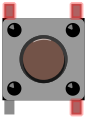
\includegraphics[height=1in]{images/Button.png}}
\label{ris:image}
\end{figure}

Кнопки з 4 контактами можна розглядати як 2 пари рельс, що з'єднуються під час натиснення.

\begin{tikzpicture}[scale=1.5]		
	\draw[line width=2] (0,0.5) -- (0.5,0.5) -- (0.5, -0.5) -- (0, -0.5);
	\draw[line width=2] (0.5,0) -- (0.7,0) -- (1.5, 0.3);
	\draw[line width=2] (1.5,0) -- (1.7,0);
	\draw[line width=2] (2.2, 0.5) -- (1.7, 0.5) -- (1.7, -0.5) -- (2.2, -0.5);	
\end{tikzpicture}

\begin{tikzpicture}[scale=1.5]		
	\draw[line width=2] (0,0) -- (0.7,0) -- (1.4, 0.4);
	\draw[line width=2] (1.4,0) -- (2.1,0);
	\draw [black, fill=black] (0.7,0) circle [radius=0.07];
	\draw [black, fill=black] (1.4,0) circle [radius=0.07];
\end{tikzpicture}	

Під час замикання та розмикання контактів кнопки між пласниами кнопки виникають мікроіскри, за рахонок чого відбуваються десятки перемикань за декілька мілісекунд. Це явице називається "дрижанням" (англ. \textit{bounce}). Цей ефект потрібно враховувати якщо потрібно фіксувати натиснення.

Поки кнопка натиснута, вихідна напруга $V_{out} = V_{cc}$, але коли вона відпущена, $V_{out} \neq 0$. Кнопка і провідники в цьому випадку працюють як антена, і $V_{out}$ буде «шуміти», приймаючи випадкові значення «з повітря».

Поки з'єднання немає, необхідно створити резервний шлях для визначення напруги. Для цього використовують один з двох варіантів.

\begin{figure}[h!]
\caption{Схема з стягуючим резистором}
\center{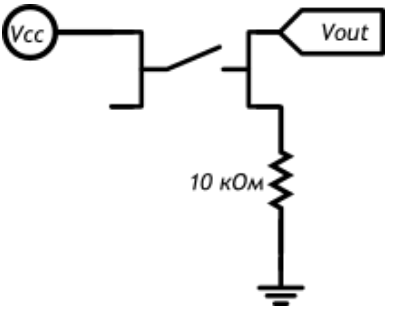
\includegraphics[height=2in]{images/ButtonShceme1.png}}
\label{ris:image}
\end{figure}

Якщо є натиснення: $V_{out} = V_{cc}$.

Якщо немає натиснення: $V_{out} = 0$.


\begin{figure}[h!]
\caption{Схема з підтягуючим резистором}
\center{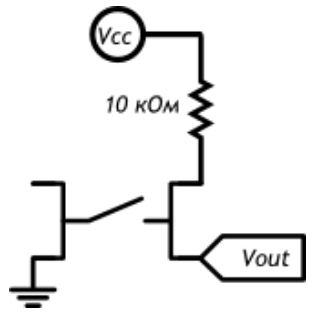
\includegraphics[height=2in]{images/ButtonShceme2.png}}
\label{ris:image}
\end{figure}

Якщо є натиснення: $V_{out} = 0$.

Якщо немає натиснення: $V_{out} = V_{cc}$.

\subsection{Широтно-імпульсна модуляція}

Мікроконтролери зазвичай не можуть видавати довіну напругу. Вони можуть видати або напругу живлення (наприклад, $5\text{В}$), або землю (тобто $5\text{В}$).

Але рівнем напруги можна управляти багатьма присторями: наприклад, яскравість світлодіода або швидкість обертання мотора. Для симуляції неповної напруги використовується ШІМ (Широтно-Імпульсна Модуляція, англ. \textit{Pulse Width Modulation} або просто \textit{PWM}).

Вихід мікроконтролера перемикається між землею і $V_{cc}$ тисячі разів в секунду. Або, як ще кажуть, має частоту в тисячі герц. Око не помічає мерехтіння більше $50 \text{Гц}$, тому нам здається, що світлодіод не мерехтить, а горить в півсили.

Аналогічно, розігнаний мотор не може зупинити вал за мілісекунди, тому ШІМ-сигнал змусить обертатися його в неповну силу.

\subsection{Дільник напруги}

Послідовно підключені резистори ділять напругу, що надходить на них у певній пропорції.

Сила струму, що протікає через резистори однакова, тому що вони з'єднані послідовно, і по закону Ома може бути розрахована як:

$$ I = \dfrac{V_{CC}}{R_1 + R_2} $$

За тим же законом Ома можна обчислити напругу $V_{out}$, яке падає на резисторі $R_2$:

$$ V_{out} = U_2 = I \cdot R_2 = \frac {R_2 \cdot V_{CC}}{R_1 + R_2} $$

З отриманої формули видно, що чим більше $R_2$ щодо $R_1$, тим більша напруга падає на ньому.

\paragraph{Зчитування резистивних сенсорів.}

Якщо замість $R_2$ використовувати не постійний резистор, а датчик, який змінює свой опір, $V_{out}$ буде залежати від вимірюваного значення.

\begin{figure}[h!]
\center{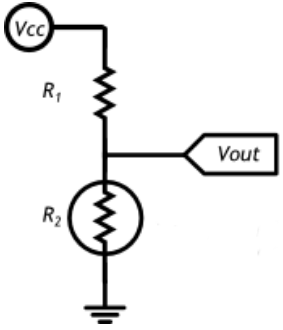
\includegraphics[height=2in]{images/VoltageDivider.png}}
\label{ris:image}
\end{figure}

Використовуючи мікроконтролер можна вимірювати напругу. Таким чином, можна використовувати властивості дільника напруги для отримання показань від сенсора.

\paragraph{Приклади резистивних датчиків}
\subparagraph{Термістор}
змінює свій опір залежно від власної температури.

\begin{figure}[h!]
\center{
\includegraphics[height=1in]{images/Termistor.png}}
\label{ris:image}
\end{figure}

\begin{tikzpicture}[scale=2]		
	\draw[line width=2] (0,0) -- (0.3,0) -- (0.4,0.1) -- (0.5, -0.1) -- (.6, 0.1) -- (.7, -0.1) -- (.8, 0.1) -- (.9, -0.1) -- (1,0) -- (1.3, 0);
	\draw[line width=2] (0.55, -0.2) -- (0.75, 0.2) -- (1.2, 0.2);
\end{tikzpicture}

\subparagraph{Фоторезистор}
змінює свій опір залежно від сили світла, що потрапляє на його керамічну "змійку".
\begin{figure}[h!]
\center{
\includegraphics[height=0.5in]{images/Photoresistor.png}}
\label{ris:image}
\end{figure}

\begin{tikzpicture}[scale=2]		
	\draw[line width=2] (0,0) -- (0.3,0) -- (0.4,0.1) -- (0.5, -0.1) -- (.6, 0.1) -- (.7, -0.1) -- (.8, 0.1) -- (.9, -0.1) -- (1,0) -- (1.3, 0);
	\draw[line width=2] (0.65,0) circle (0.4);
	\draw[->, line width=2] (1.05, .75) -- (0.76, .41);
	\draw[->, line width=2] (1.2, .7) -- (0.9, .35);
\end{tikzpicture}

\subparagraph{Потенціометр}
ще називають змінним резистором, тримерами. Це дільник з двох резисторів в одному корпусі. Тому у нього 3 ноги: харчування, вихід, земля.
\begin{figure}[h!]
\center{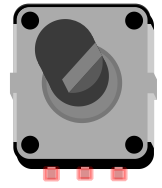
\includegraphics[height=1in]{images/POT.png}}
\label{ris:image}
\end{figure}

\begin{tikzpicture}[scale=2]		
	\draw[line width=2] (0,0) -- (0.3,0) -- (0.4,0.1) -- (0.5, -0.1) -- (.6, 0.1) -- (.7, -0.1) -- (.8, 0.1) -- (.9, -0.1) -- (1,0) -- (1.3, 0);
	\draw[line width=2] (0.75, 0.2) -- (1.2, 0.2);
	\draw[->, line width=2] (0.75, 0.2) -- (0.49, -0.3);
\end{tikzpicture}

Співвідношення $R_1$ і $R_2$ змінюється поворотом ручки. Від $100\%$ на користь $R_1$ до $100\%$ на користь $R_2$.

\subsection{Біполярний транзистор}

Транзистор~-- це електронна кнопка. На кнопку натискають пальцем, а на біполярний транзистор~-- струмом.

\begin{figure}[h!]
\center{
\includegraphics[height=1in]{images/BipolarTransistor.png}}
\label{ris:image}
\end{figure}

\begin{tikzpicture}[scale=1]		
	\draw[line width=2] (0,0) -- (1.6,0);
	\draw[line width=2] (1.6,0.7) -- (1.6,-0.7);
	\draw[line width=2] (2.5,1.5) -- (2.5,0.84) -- (1.6, 0);	
	\draw[line width=2] (2,0) circle (1);
	\draw[line width=2] (2.5,-0.84) -- (2.5,-1.5);
	\draw[->, line width=2] (1.6, 0) -- (2.5, -0.84);
	\node[below left, text=gray] at (1,0) {Б};
	\node[right, text=gray] at (2.5,1) {К};
	\node[right, text=gray] at (2.5,-1.1) {E};	
\end{tikzpicture}

Транзистори використовують для управління потужними джерелами струму за допомогою слабких сигналів з мікроконтролера.

Нога, що виконує роль «кнопки» називається база (англ. \textit{base}).
Поки через базу тече невеликий струм, транзистор відкритий:
Великий струм може втікати в колектор (англ. \textit{collector}) і витікати з емітера (англ. \textit{emitter})

\paragraph{Основні характеристики}
\begin{center}
\begin{tabular}{|l|c|c|}
\hline
\textit{Назва} & \textit{Позначення} & \textit{Одиниці виміру} \\
\hline
Максимальна напруга колектор-емітер & $V_{CE}$ & Вольт \\
\hline		
Максимальний струм через колектор & $I_C$ & Ампер \\
\hline
Коефіцієнт посилення & $h_{fe}$ & ~ \\
\hline
\end{tabular}
\end{center}

Типова схема підключення

Транзистор підсилює максимально допустимий струм в $h_{fe}$ раз:

$$ I_{CE} = I_{BE} \cdot h_{fe} $$

Приклад розрахунку

Якщо керуючий сигнал на базі транзистора з $h_{fe}$ і резистором номіналом $1 \text{кОм}$ становить $5 \text{В}$:

Який максимальний струм зможе пропустити через себе транзистор ($I_{BE}$)?

Яким за величиною буде керуючий струм ($I_{CE}$)?

$V_B = 5\text{В}$,
$R = 1\text{кОм}$,
$h_{fe} = 50$.


$ I_{BE} = \dfrac{V_B}{R} = \dfrac{5\text{В}}{1000\text{Ом}} = 5 \cdot 10^{-3} \text{А} $.

$I_{CE} = I_{BE} \cdot h_{fe} = 250 \cdot 10^{-3} \text{А}$.

Отже, якщо на базу подається $5\text{В}$ через резистор в $1\text{кОм}$, транзистор відкриється настільки, що зможе пропустити до $250\text{мА}$. При цьому керуючий струм складе всього $5\text{мА}$.

\subsection{Польовий транзистор}

Польовий MOSFET-транзистор~-- ключ для управління великими струмами за допомогою невеликого напруги.

\begin{figure}[h!]
\center{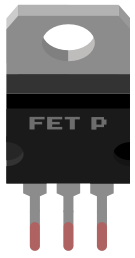
\includegraphics[height=1in]{images/PoleTransistor.png}}
\label{ris:image}
\end{figure}

\begin{tikzpicture}[scale=1]		
	\draw[line width=2] (0, -0.7) -- (1.7,-0.7) -- (1.7,0.7);
	\draw[line width=2] (2.5,1.5) -- (2.5,0.7) -- (1.9, 0.7);	
	\draw[line width=2] (2,0) circle (1);
	\draw[line width=2] (1.9, -0.7) -- (2.5,-0.7) -- (2.5, -1.5);
	\draw[->, line width=2] (2.5, 0) -- (1.9, 0);
%	\draw[densely dashed, line width=2] (1.9, 0.7) -- (1.9, -0.7);

	\draw[line width=2] (1.9, -0.7) -- (1.9,-0.4);
	\draw[line width=2] (1.9, 0.7) -- (1.9,0.4);
	\draw[line width=2] (1.9, 0.25) -- (1.9, -0.25);

	\node[below left, text=gray] at (1,0) {З};
	\node[right, text=gray] at (2.5,1) {С};
	\node[right, text=gray] at (2.5,-1.1) {В};	
\end{tikzpicture}

"Кнопка" називається затвором (англ. \textit{gate}). Поки на затворі є невелика напруга, транзистор відкритий: великий струм може втікати в стік (англ. \textit{drain}) і витікати з витоку (англ. \textit{source}).

На відміну від біполярного транзистора польовий контролюється саме напругою, а не струмом. Тобто у відкритому стані струм через затвор не проходить.

Використовуйте MOSFET для управління великими струмами, від сотень міліампер, коли біполярного транзистора вже не досить.

\paragraph{Основні характеристики}
\begin{center}
\begin{tabular}{|l|c|c|}
\hline
\textit{Назва} & \textit{Позначення} & \textit{Одиниці виміру} \\
\hline
Максимальна напруга стік-витік & $V_{DS}$ & Вольт \\
\hline		
Максимальний струм через стік & $I_D$ & Ампер \\
\hline
Опір стік-витік & $R_{DSon}$ & Ом \\
\hline
Потужність, що розсіюється & $P_D$ & Ватт \\
\hline
\end{tabular}
\end{center}

Транзистор не ідеальний і частина пропускної потужності перетворюється в тепло.

$ P_H = I^2 \cdot R_{DSon} $

Якщо $P_H$ перевищить $P_D$, без використання додаткового охолодження транзистор згорить.

\subsection{П'єзодинамік}

П'єзогенератор звуку (англ. \textit{buzzer}) переводить змінну напругу в коливання мембрани, яка в свою чергу створює звукову хвилю. П'єзодинамік~-- це конденсатор, який звучить при зарядці і розрядці.

\paragraph{Основні характеристики}
\begin{center}
\begin{tabular}{|l|c|c|}
\hline
\textit{Назва} & \textit{Позначення} & \textit{Одиниці виміру} \\
\hline
Номінальна напруга & $V$ & Вольт \\
\hline		
Гучність (на заданій відстані) & $P$ & Децибел \\
\hline
Пікова частота & $f_P$ & Герц \\
\hline
Ємність & $C$ & Фарад \\
\hline
\end{tabular}
\end{center}

\paragraph{Підключення з регулюванням гучності.} 

За допомогою потенціометра можна зменшити струм за рахунок чого зменшиться гучність.
За допомогою ризистора можна вирівняти напругу поки транзистор закритий.

\begin{figure}[h!]
\center{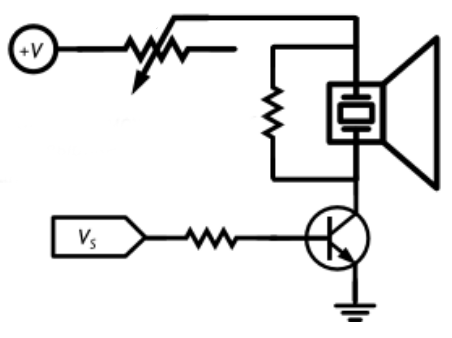
\includegraphics[height=2.5in]{images/BuzzerConnection.png}}
\label{ris:image}
\end{figure}

\subsection{Мотор}

Мотор перетвроює електричну енергію в механічну енергію обертання.

\begin{figure}[h!]
\center{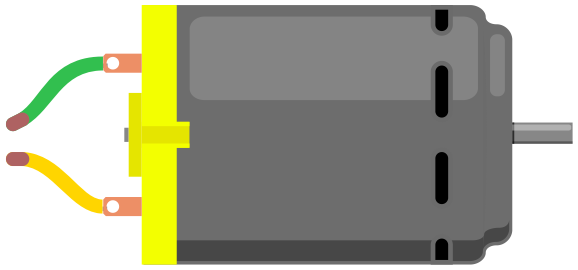
\includegraphics[height=1in]{images/Motor.png}}
\label{ris:image}
\end{figure}

\begin{tikzpicture}[scale=1]		
	\draw[line width=2] (0, 0) -- (0, 1);
	\draw[line width=2] (0, 3) -- (0, 4);
	\draw[line width=2] (0, 2) circle (1);
	\node[scale=3] at (0, 2) {M};
\end{tikzpicture}

Найпростіший вид мотора~-- колекторний. При подачі напруги в одному напрямку вал крутиться за годинниковою стрілкою, в зворотному напрямку~-- проти годинникової.

\paragraph{Основні характеристики}
\begin{center}
\begin{tabular}{|l|c|c|}
\hline
\textit{Назва} & \textit{Позначення} & \textit{Одиниці виміру} \\
\hline
Номінальна напруга & $V$ & Вольт \\
\hline		
Струм споживання без навантаження & $I_F$ & Ампер \\
\hline
Струм споживання при блокуванні & $I_S$ & Ампер \\
\hline
Швидкість обертання без навантаження & $\omega$ & $c^{-1}$ \\
\hline
Максимальний крутний мометн & $\tau$ & Н$\times$м \\
\hline
\end{tabular}
\end{center}

Мотори~-- потужні споживачі з рядом побічних ефектів. Для управління ними необхідні додаткові компоненти.

Для використання мотора доцільніше використовувати додаткове джерело живлення з рекомендованою для мотора напругою (+9V).
За допомогою транзистора можна управляти потужним моторм за допомого слабкого сигналу $V_S$.
ШІМ-сигнал використовують для регулювання швидкістю обертання вала.
Під час роботи мотор створює електромагнітні шуми. Використання конденсатора дозволяє згладити пульсації.
Коли відбувається гальмування мотора, він працює як генератор, створюючи напругу зворотної полярності. Діод потрібен для пропускання утвореного струму чез себе. Без діода вийде з ладу керуючий транзистор.

\begin{figure}[h!]
\center{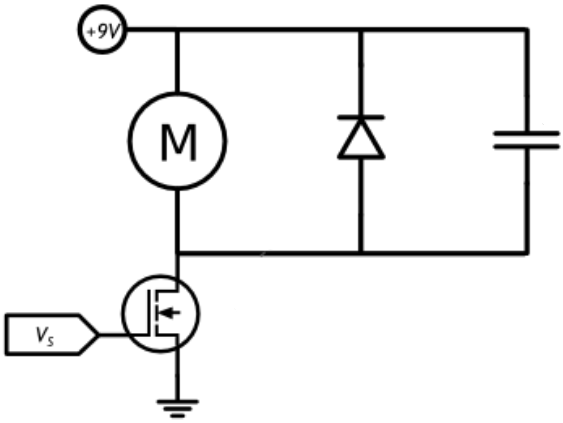
\includegraphics[height=3in]{images/MotorConnection.png}}
\label{ris:image}
\end{figure}
%=================================================

\chapter{Основи роботи з Arduino}

\section{Arduino}

Що таке Arduino?

Arduino - це open-source платформа, яка складається з двох основних частин: самої плати (часто званої мікроконтролер) і програмного забезпечення (спеціальної оболонки для програмування плати) або IDE (Integrated Development Environment). Програмне забезпечення запускається на персональному комп'ютері і дозволяє записувати розроблений вами код на плату.
Загальна інформація про Arduino

Arduino знайшли особливо сильну популярність серед людей, які тільки починають займатися електронікою. На те є кілька причин. На відміну від більшості попередників, Arduino не вимагає додаткового обладнання (програматора) для завантаження коду на плату - використовується простий USB-кабель. Оболонка для програмування - Arduino IDE використовує спрощену версію C ++, що полегшує процес навчання для новачків. Крім того, Arduino використовує стандартизований форм фактор для більшості своїх плат, завдяки чому з'явився цілий комплект додаткових "Шілд".

Arduino Uno показана на малюнку нижче:

Arduin Uno

Arduino Uno - одна з найпопулярніших плат в лінійці і є відмінним вибором для початківців. Технічні характеристики цієї моделі будуть розглянуті нижче.

Оболонка Arduino IDE:

Arduino IDE

Чи повірите чи ні, але показані на малюнку вище 10 рядків коду достатньо, щоб змусити блимати вбудований на плату світлодіод. Можливо, сам код для вас зараз не дуже зрозумілий, але повірте, він гранично логічний і лаконічний. Після цієї статті і декількох туторіали, вам не складе труднощів його реалізувати самостійно.

У цій статті ми зупинимося на таких основних моментах:

    Які проекти можна реалізувати з Arduino
    Основні вузли плат Arduino
    Номенклатура найвдаліших моделей Arduino
    Додаткові (периферійні) пристрої для Arduino

Рекомендуємо також додатково почитати

Arduino призначена не тільки для вузькоспеціалізованих фахівців. При цьому процес їх освоєння буде набагато легше і приємніше, якщо у вас за плечима базові знання схемотехніки і електротехніки. Рекомендуємо отримати хоча б загальне розуміння перерахованих нижче речей перш ніж заглиблюватися в дивовижний світ Arduino:

    Що таке електрика?
    Закон Ома
    Електричний ланцюг
    Інтегральна схема (мікросхема)
    аналоговий сигнал
    цифровий сигнал

Навіщо вам Arduino?

Arduino розроблена для ... Всіх. Так, у всякому разі, заявлено на офіційному сайті компанії. Список приблизно такий: артисти, дизайнери, хакери, програмісти, інженери, для всіх, хто цікавиться розробкою і втіленням інтерактивних проектів. Arduino може взаємодіяти з кнопками, світлодіодами, двигунами, динаміками, GPS-модулями, температуру, камерами, інтернетом і навіть вашим смартфоном або телевізором! Подібна гнучкість в поєднанні з тим, що софт від Arduino - абсолютно безкоштовний, самі плати досить дешеві і легкі в освоєнні привела до появи величезної спільноти шанувальників даної платформи, які викладають власні шматки коду, бібліотеки та інструкції для величезної кількості проектів з використанням Arduino.

Arduino використовуються в якості "мізків" для роботів, 3D принтерів, в системах автоматизованого поливу, світлодіодних кубах, грілках, в системах "розумних будинків" і т.д. Список постійно зростає. Всі проекти і не перерахуєш. Скажімо так: Arduino знаходять застосування практично в будь-якому проекті, де необхідна автоматизація.

Arduino\_Game\_Pad\_Project

І це тільки вершина айсберга. Якщо вам цікаво поглянути на Arduino проекти в дії, ось кілька посилань на хороші ресурси (англійською мовою):

    Instructables
    Bildr
    Arduino Playground
    The ITP Physical Computing Wiki
    LadyAda
    Make: Projects

З чого складається плата Arduino?

Випускаються різні моделі Arduino. Кожна з них "заточена" для різних завдань. Деякі плати принципово відрізняються від наведеної на малюнку нижче. Але більшість з них мають такі однакові вузли:

Arduino Uno - опис
Роз'єм живлення (USB / роз'єм для адаптера)

Кожна плата Arduino повинна приєднуватися до джерела живлення. Arduino Uno може живитися від USB кабелю від вашого персонального комп'ютера Або від окремого адаптера, який підключається до передбаченого на платі роз'єму. На малюнку з'єднання через USB відзначено (1), а роз'єм для зовнішнього джерела живлення - (2).

USB також використовується для завантаження вашої програми (скетчу) на плату.

Примітка! Не використовуйте джерело живлення з напругою на виході більше 20 вольт. Це може привести до того, що ваша плата перегорить. Рекомендоване напруга живлення для Arduino - від 6 до 12 вольт.
Роз'єми (Піни) (5V, 3.3V, GND, Analog, Digital, PWM, AREF)

Піни на вашій платі Arduino - це передбачені роз'єми, до яких ви будете підключати дроти від периферійних пристроїв (дуже часто для прототипів використовують монтажні плати (макетна плата, макетке) і дроти з коннекторами на кінцях). На Arduino кілька типів пинов, кожен з яких підписаний відповідно до виконуваної функцією.

    GND (3): скорочення від 'Ground' - 'Земля'. На платах кілька пинов GND, кожен з яких може використовуватися для заземлення вашої електричного кола.
    5V (4) і 3.3V (5): як ви могли вже здогадатися - піти, які на виході забезпечують харчування 5 вольт і 3.3 вольт відповідно. Більшість компонентів, які підключаються до Arduino, благополучно харчуються саме від 5 або 3.3 вольт.
    Analog (6): на ділянці, який підписаний 'Analog In' (від A0 до A5 на Arduino Uno) розташовані аналогові входи. Ці Піни дозволяють зчитувати сигнали від аналогових датчиків (наприклад, датчик температури) і перетворювати їх в цифрові значення, якими ми надалі оперуємо.
    Digital (7): навпроти аналогових пинов знаходяться цифрові Піни (від 0 до 13 на Arduino Uno). Ці Піни використовуються для цифрових вхідних (input) сигналів (наприклад, натискання кнопки) і для генерації цифрових вихідних (output) сигналів (наприклад, харчування світлодіода).
    PWM (8): ви напевно помітили знак (~) поряд з деякими цифровими пинами (3, 5, 6, 9, 10, і 11 на UNO). Ці Піни працюю як в звичайному цифровому режимі, так і в режимі ШІМ-модуляції (PWM). Якщо пояснити коротко - ці Піни можуть імітувати аналоговий вихідний сигнал (наприклад, для поступового згасання світлодіода).
    AREF (9): Цей пін використовується досить рідко. У деяких випадках це підключають в схему для установки максимального значення напруги на аналогових входах (від 0 до 5 вольт).

Кнопка скидання (Reset Button)

Як і на оригінальних Nintendo, на Arduino є кнопка скидання (reset) (10). При натисканні на неї контакт скидання замикається з землею і код, завантажений на Arduino починає відпрацьовувати заново. Корисна опція, якщо ваш код відпрацьовує без повторів, але ви хочете протестить його роботу.
Індикатор живлення (Power LED)

Трохи праворуч і нижче написи "UNO" встановлений світлодіод, підписаний "on" (11). Цей світлодіод повинен загорітися, коли ви підключили Arduino до джерела живлення. Якщо світлодіод не зайнявся - поганий знак;).
Світлодіоди TX і RX

TX - скорочення від transmit (передача), RX - від receive (прийом). Ці умовні позначення часто зустрічаються в електроніці для позначення контактів, які відповідають за серійний обмін даними. На Arduino Uno ці контакти зустрічаються два рази на цифрових пінах 0 і 1 і в якості світлодіодів TX і RX (12). Ці світлодіоди дозволяють візуально відслідковувати, передає або приймає дані Arduino (наприклад, при завантаженні програми на плату).
Головна інтегральна мікросхема (IC)

Чорна деталь з металевими коннекторами з двох сторін це інтегральна мікросхема, мікропроцесор (IC або Integrated Circuit) (13). Можете сміливо вважати, що це "мізки" нашої Arduino. Цей чіп різний в різних моделях Arduino, але зазвичай він відноситься до лінійки мікропроцесорів ATmega від компанії ATMEL. Це може виявитися важливою інформацією для завантаження скетчу на плату. Модель інтегральної мікросхеми зазвичай вказана на її верхній корпусних частини. Для додаткової інформації про вашу мікросхемі варто звернутися до її даташіту.
Регулятор напруги

Регулятор напруги (14) is виконує функцію, вказану в назві - контролює напругу, яка надходить на плату Arduino. Можете його собі уявити як охоронця, який не пропускає занадто велика напруга на плату, щоб уникнути її ушкоджень. Звичайно ж, у регулятора є своя межа. Так що живити Arduino напругою більше 20 вольт не можна.
Номенклатура плат Arduino

Arduino виробляє різні плати, кожна з який має власні особливості. Крім того, Arduino дотримуються моделі open source, завдяки чому інші можуть модифікувати і виробляти клони Arduino, розширювати і змінювати їх функціонал і форм-фактор. Нижче наведені короткі відомості про різні моделі Arduino.
Arduino Uno (R3)

Arduino Uno - відмінний вибір для початківців. Дуже збалансована плата, на якій є, все, що вам може знадобитися і мінімум зайвого. На платі 14 цифрових пинов, які працюю на вхід і на вихід (6 з них підтримують ШІМ-модуляцію), 6 аналогових входів. Підключається плата за допомогою USB. Є джек для окремого джерела живлення, кнопка скидання і т.п. Для початку роботи з мікро контролером достатньо підключити плату до комп'ютера за допомогою USB кабелю.

Arduino Uno R3
LilyPad Arduino

Основна плата в лінійки LilyPad Arduino! LilyPad розроблена в першу чергу для використання на одязі. Піни з'єднуються з периферійними пристроями за допомогою струмопровідної нитки. Є купа додаткових плат розширень для LilyPad. Більшість з них спроектовані таким чином, що не бояться вологи.

LilyPad Arduino

Основна плата в лінійки LilyPad Arduino! LilyPad розроблена в першу чергу для використання на одязі. Піни з'єднуються з периферійними пристроями за допомогою струмопровідної нитки. Є купа додаткових плат розширень для LilyPad. Більшість з них спроектовані таким чином, що не бояться вологи.

LilyPad Arduino
RedBoard

Розробка SparkFun, яка програмується за допомогою USB Mini-B кабелю в оболонці Arduino IDE. Основними перевагами виробник називає: стабільність роботи під ОС Windows 8 завдяки драйверам з необхідною цифровим підписом. На платі використовується чіп USB / FTDI, який менше за габаритами в порівнянні з чіпом на Arduino UNO. Для заливки скетчу на плату в IDE вибирається модель Arduino UNO. Регулятор напруги розрахований на харчування в діапазоні від 7 до 15 вольт.

RedBoard Arduino
Arduino Mega (R3)

Arduino Mega - немов старший брат Uno. На платі багато (54!) Цифрових входів / виходів (14 з них підтримують ШІМ-модуляцію). Завдяки великій кількості пінів, плата використовується для комплексних проектів, в яких підключається велика кількість периферії (наприклад, сведодіодов або кнопок). Підключення до комп'ютера реалізується таким же кабелем як і на Arduino Uno. Природно, передбачений джек для адаптера.

Arduino Mega
Arduino Leonardo

Leonardo - перша розробка Arduino, в якій використовується один мікроконтролер із вбудованим USB. Це означає, що плата стає простіше і дешевше. Так як плата підключається безпосередньо до USB без конвертера, є бібліотеки, які дозволяють емулювати комп'ютерну мишу, клавіатуру і багато іншого!

Arduino Leonardo
Arduino Pro Mini

Arduino Pro Mini - найкращий варіант для ваших проектів, в яких необхідна висока мобільність або кріплення контролера безпосередньо на рухомих вузлах вашого механізму. Повний гайд по використанню плат Arduino Pro Mini можна знайти в цій статті.

Arduino Pro Mini
Додаткові пристрої для Arduino

Безумовно, Arduino сама по собі вже прекрасна. Але як окремий вузол вона на багато що не здатна. Щось треба до неї підключати. На просторах інтернету величезна кількість туторіали і проектів, з яких ви можете черпати ідеї для своїх проектів. У цій частині ми зробимо невеликий огляд датчиків і Шілд (плат розширень) для Arduino.
Датчики (сенсори)

За допомогою коротенького коду і Arduino ви можете управляти найширшим спектром датчиків - сенсорів, які дозволяють вимірювати рівень освітленості, температуру, тиск, відстань, силу, вологість, радіоактивність, прискорення і багато іншого. На малюнку нижче наведено кілька з величезної кількості датчиків, сумісних з Arduino:

датчики Arduino
Шілд (Shields) для Arduino

Крім усього іншого, є така чудова річ як Шілд - по суті це окрема схема живлення, яка має коннектори і сідає на вашу плату Arduino і забезпечує спрощене управління двигунами (Motor Шилд), підключення до інтернету (Ethernet Шилд), радіозв'язок, управління рідкокристалічними і сенсорними екранами і т.д.

\section{Arduino IDE}

\section{Fritzing}

\chapter{Програмування в середовищі\\Arduino IDE}

\section{Змінні}

\subsection{Типи даних}

Комп'ютери та Arduino в тому числі, працюють з різними типами даних. В їх основі лежить арифметично-логічний пристрій (АЛП), що виконує арифметичні і логічні операції з клітинками пам'яті: $R1 + R2$, $R3 * R7$, $R4 \& R5$ і т.д. Для АЛП немає різниці, який тип даних відображати користувачеві: текст, цілі числа, числа з плаваючою комою або навіть частина програмного коду.

Команди для цих операцій надходять від компілятора, а команди компілятору передаються від користувача. Саме програміст, визначає для компілятора, що це значення~-- ціле, а інше значення - число з плаваючою комою.

\paragraph{Характеристика основних типів даних в Arduino IDE}

Оболонка для програмування Arduino по суті являє з себе мову \code{C++} з підтримкою великої кількості бібліотек для полегшення процесу написання програм. \code{C++} пропонує широкий вибір різних типів даних.

Нижче представлений список основних типів даних, які використовуються в скетчах Arduino. Поруч з кожним типом даних вказано його розмір. Зверніть увагу, сто змінні типу \code{signed} дають можливість оперувати позитивними і від'ємними числами, а змінні типу \code{unsigned} допускають тільки роботу з додатними значеннями.

    \code{boolean} (8 біт)~-- просте логічне \code{true / false}
    
    \code{byte} (8 біт)~-- \code{unsigned} число в діапазоні від $0-255$
    
    \code{char} (8 біт)~-- \code{signed} число в діапазоні від $-128$ до $127$. У деяких випадках компілятор буде інтерпретувати цей тип даних як символ, що може призвести до несподіваних результатів.
    
    \code{unsigned char} (8 біт)~-- то ж що і \code{byte}; для ясності коду рекомендується замість цього типу даних використовувати \code{byte}.
    
    \code{word} (16 біт)~-- \code{unsigned} число в діапазоні від $0$ до $65535$
    
    \code{unsigned int} (16 біт)~-- те саме, що і \code{word}. Рекомендується замінювати типом даних \code{word} для скорочення коду і ясності
    
    \code{int} (16 біт)~-- \code{signed }число в діапазоні від $-32768$ до $32767$. Один з найпоширеніших типів даних, який дуже часто використовується для оголошення змінних в скетчах-прикладах для Arduino, вбудованих в Arduino IDE
    
    \code{unsigned long} (32 біта)~-- \code{unsigned} число в діапазоні від $0-4,294,967,295$. Найчастіше цей тип даних використовується для зберігання результатів функції \code{millis()}, яка повертає кількість мілісекунд, протягом якого виконувалась дастина коду.
    
    \code{long} (32 біта)~-- \code{signed} число в діапазоні від $-2,147,483,648$ до $2,147,483,647$
    
    \code{float} (32 біта)~-- \code{signed} число в діапазоні від $-3.4028235\cdot 10^{38}$ до $3.4028235\cdot 10^{38}$. Числа з плаваючою комою не характерні для Arduino і компілятору доведеться довше опрацьовувати дані. Так що рекомендується за можливості їх уникати.


\section{Структури}

\subsection{Базовий код для програмування план Arduino}
Функція  \code{setup()} викликається на початку скетчу. Вона використовується для ініціалізації змінних, настройки режимів роботи пінів (на введення або на виведення). Функція \code{setup()} виконується один раз після подачі живлення або перезавантаження плати Arduino.

Після виконання функції \code{setup()}, циклічно виконується функція \code{loop()}, яка безпосередньо є основою програми для управління платою Arduino.

Код, наведений нижче, не виконує ніяких завдань, але його структура корисна як база для всіх програм. Крім того, зверніть увагу на те, як залишаються коментарі в скетчах.

Кожен рядок, який починається з (\code{//}) не читатися компілятором, так що у ньому можна записувати будь-які дані.


\newpage

Програмний код:

\begin{lstlisting}[label=some-code,caption=Структура програми]
int void() {
	for (int i=0; i<5; i++) {
		while (true) {
			docool();		
		}	
	}
// коментарі українською
}
\end{lstlisting}	

\subsection{Умовний оператор}

Вираз \code{if()} є основним для всіх керуючих структур в програмуванні. Цей вираз дозволяє вам здійснювати чи ні певним чином впливати залежно від умови, що є \code{true} (виконується) або \code{false} (не виконується). Синтаксис умови \code{if} виглядає наступним чином:

\begin{lstlisting}[label=conditionoperator,caption=Умовний оператор (неповна форма)]
if (someCondition) {
	// дії, які потрібно виконати, якщо умова виконується
}
\end{lstlisting}

Так само є подібні варіації структури з використанням if-else. Виглядає це наступним чином:

\begin{lstlisting}[label=conditionoperator,caption=Умовний оператор (повна форма)]
if (someCondition) {
	// дії, які потрібно виконати, якщо умова виконується
}
else {
	// дії, які потрібно виконати, якщо умова не виконується
}
\end{lstlisting}

Також є структура else-if, за допомогою якої ви можете перевірити друга умова, якщо перше не виконується:

\begin{lstlisting}[label=conditionoperator,caption=Умовний оператор (декільки умов)]
if (someCondition) {
	// дії, які потрібно виконати, якщо умова виконується
} 
else if (anotherCondition) {
	// дії, які потрібно виконати тільки якщо не виконується перша умова
	// а друга умова виконується
}
\end{lstlisting}

Кількість розгалужень може бути необмеженою.

\subsection{Оператор вибору}

\code{switch}

\subsection{Циклічні оператори}
Циклічні оператори використовуються для повтоерння однакових або однотипних дій.

\paragraph{for}

Доцільно використовувати коли відома кількість поврень, які потрібно виконати.

\begin{lstlisting}[label=conditionoperator,caption=Оператор повторення for]
for(int i=0; i<10; i++) {
	// всі оператори всередині фігурних дужок називаються тілом циклу
	Serial.println(i);
}
\end{lstlisting}

Перший аргумент~-- початкове значення лічильника. В даному випадку стоврюється внутрішня змінна \code{i}, якій надається початкового значення 0.

Другий аргумент~-- умова за якої тіло циклу виконується. Зазвичайумова вказується як заежність від лічильника. У прикладі тіло циклу виконуватиметься поки значення лічильника буде меншим за 10.

Третій аргумент~-- спосіб зміни лічильника. У прикладі лічильник з кожною ітерацією збільшується на 1. Таким чином, враховуючи умову, тіло циклу викорається 10 разів.

Кожен аргумент не є обов'язковим і може бути пропущений під час оголошення циклу. Але для коректної роботи потрібно конторювати всі складові окремо. Навдемо приклад тієї ж програми з порожніми агрументами.

\begin{lstlisting}[label=conditionoperator,caption=Оператор повторення for]
int i = 0; // оголошення та ініціалізація лічильника за межами циклу
for(;;) {
	Serial.println(i);
	i++; // зміна значення лічильника
	if (i >= 10) break;
}
\end{lstlisting}

Для аналогічної роботи такої циклічної структури використовується оператор \code{break}, який потрібен для дострокового переривання виконання циклу.

\paragraph{Цикл while}
\paragraph{Цикл do...while}

\subsection{Масиви}

Масив~-- це набір однотипних змінних, доступ до яких здійснюється через їх індекс. У мові програмування C, на якому заснований Arduino, масиви можуть бути досить складними.

\paragraph{Створення (оголошення) масиву.} 
Всі методики, представлені нижче, підходять для створення (оголошення) масиву.

\begin{lstlisting}[label=conditionoperator,caption=Оголошення масиву]
int myInts [6];
int myPins [] = {2, 4, 8, 3, 6};
int mySensVals [6] = {2, 4, -8, 3, 2};
char message [6] = "hello";
\end{lstlisting}

Ви можете оголосити масив без його ініціалізації як \code{myInts}.

У \code{myPins} оголошується масив без безпосередньої вказівки розміру. Компілятор вважає кількість елементів і створює масив відповідного розміру.

Можна одночасно форматувати і вказати розмір вашого масиву, як, наприклад, це зроблено в \code{mySensVals}. Зверніть увагу, що при оголошенні масиву типу \code{char}, необхідний ще один елемент для зберігання обов'язкового \code{null}-символу.

\paragraph{Доступ до елементів масиву.}
Індексація в масивах починається з нуля. Тобто, перший елемент масиву буде мати порядковий номер \code{0}. Таким чином:

\code{mySensVals [0] == 2, mySensVals [1] == 4}, і так далі

Тобто, наприклад, в масиві з десяти елементів, останній елемент буде мати індекс дев'ять. наприклад:

\code{int myArray [10] = {9,3,2,4,3,2,7,8,9,11};} 
\code{myArray[9]} містить 11, а вираз \code{myArray[10]} некоректний і містить випадкові дані (іншу адресу пам'яті).

З цієї причини треба бути акуратним при доступі до масивів. Звертаючись до елементу масиву, значення якого більше ніж оголошений розмір ви счітвиете з пам'яті значення, яке призначене для інших завдань. Зчитування таких даних просто призведе до некоректних результатів роботи програми в подальшому. Також не дуже хорошою ідеєю є запис даних в довільні місця. Крім того, відстежити цю помилку при перевірці коду теж складно.

На відміну від BASIC або JAVA, компілятор C не перевіряє, чи отримуємо ми доступ до елементу масиву в попередньо оголошених межах.

Для надання значення елементу масива під номером \code{0}:

\code{mySensVals [0] = 10;}

Для отримання значення елемента масиву за номером \code{4}:

\code{x = mySensVals [4];}

\section{Функції}

\subsection{Цифрове введення/виведення}

\subsubsection{digitalRead()}

\subparagraph{Опис:}

Читає значення \code{HIGH} або \code{LOW} з визначеного цифорового піна.
\subparagraph{Синтакс:}
\code{digitalRead(pin)}
\subparagraph{Параметри:}
\code{pin}~-- номер цифрового піна (ціле число) з якого потрібно зчитати дані.
\subparagraph{Результат виконання:}
значення \code{HIGH} або \code{LOW}, якщо є чи немає сигнал на вказаному піні відповідно.

Встановлює прочитане значення з піна 13 і зипис цього значення у пін 7.
\begin{lstlisting}[label=digitalreadwrite,caption=Використання функції digitalRead()]
int ledPin = 13;   // Світлодіод приєднано до піна 13
int inPin = 7;     // Кнопка приєнана до цифорового піна 7
int val = 0;       // Змінна для збереження отриманого значення

void setup()
{
  pinMode(ledPin, OUTPUT);      // Встановлення 13 піна для виведення
  pinMode(inPin, INPUT);        // Встановлення 7 піна для введення
}

void loop()
{
  val = digitalRead(inPin);     // зчитуємо значення на 7 піні
  digitalWrite(ledPin, val);    // встановлюємо значення для світлодіода рівним прочитаному занченню
}
\end{lstlisting}

\subparagraph{Примітки}

Якщо пін не фізично приєднано то значення функції \code{digitalRead()} може набувати випадкових значеннь \code{HIGH} або \code{LOW}.

Аналогові вхідні контакти можна використовувати як цифрові, які називаються \code{A0}, \code{A1} та ін.

\subsubsection{digitalWrite()}

\subparagraph{Опис:} Записує значення \code{HIGH} або \code{LOW} до визначеного цифорового піна.

Якщо пін-код був налаштований як \code{OUTPUT} за допомогою функції \code{pinMode()}, його напруга буде встановленf на відповідне значення: $5$В (або $3.3$В на платах $3.3$В) для значення \code{HIGH}, $0$В (земля) для \code{LOW}.

Якщо пін налаштований як \code{INPUT}, digitalWrite() активуватиме (\code{HIGH}) або вимкне (\code{LOW}) внутрішню підтяжку на вхідному піні. Рекомендується встановити \code{pinMode()} у значення \code{(INPUT\_PULLUP)} щоб увімкнути внутрішній підтягуючий резистор.

Якщо не встановилювати \code{pinMode()} в \code{OUTPUT} і підключили світлодіод до шпильки, під час виклику \code{digitalWrite(HIGH)} світлодіодний індикатор може виглядати затемненим. Без явного встановлення \code{pinMode()}, \code{digitalWrite()} буде активувати внутрішній підтягуючий резистор, який діє як обмежуючий резистор.

\subparagraph{Синтакс:} \code{digitalWrite(pin, value)}.
\subparagraph{Параметри:} \code{pin}~-- номер цифрового піна (ціле число) в який потрібно здійснити запис даних.

\code{value}~-- значення \code{HIGH} або \code{LOW}.
\subparagraph{Результат виконання:} \code{viod} (нічого).

\subparagraph{Приклад використання}

Встановлення цифрового піна $13$ в значення \code{OUTPUT} і перемикання значення з \code{HIGH} на \code{LOW} з інтервалом 1с = 1000мс.

\begin{lstlisting}[label=digitalwrite,caption=Використання функції digitalWrite()]
void setup()
{
  pinMode(13, OUTPUT);          // sets the digital pin 13 as output
}

void loop()
{
  digitalWrite(13, HIGH);       // sets the digital pin 13 on
  delay(1000);                  // waits for a second
  digitalWrite(13, LOW);        // sets the digital pin 13 off
  delay(1000);                  // waits for a second
}
\end{lstlisting}
\subparagraph{Примітки} Аналогові вхідні контакти можна використовувати як цифрові, які називаються \code{A0}, \code{A1} та ін.

\subsubsection{pinMode()}

\subparagraph{Опис:}

Налаштовує вказаний пін для введення або введення.

Як і в Arduino 1.0.1, можна ввімкнути внутрішні підсилювачі резисторів за допомогою режиму \code{INPUT\_PULLUP}. Крім того, режим \code{INPUT} явно вимикає внутрішні підказки.

\subparagraph{Синтакс:} \code{pinMode(pin, mode)}
\subparagraph{Параметри:}
\code{pin}~-- номер піна, режим якого потрібно встановити.
\code{mode}: \code{INPUT, OUTPUT} або \code{INPUT\_PULLUP}.

\subparagraph{Результат виконання:} \code{viod} (нічого).

\subparagraph{Приклад використання} див. скетч \hyperref[digitalwrite]{\code{digitalwrite()}}.

\subparagraph{Примітки} Аналогові вхідні контакти можна використовувати як цифрові, які називаються \code{A0}, \code{A1} та ін.

\subsection{Аналогове введення/виведення}

\subsubsection{analogRead()}

\subparagraph{Опис:}

Читає значення з вказаного аналогового піна. Плата Arduino містить 6 каналів (8 каналів на Mini і Nano, 16 на Mega), 10-бітний аналого-цифровий перетворювач. Це означає, що він буде перетворювати вхідну напругу від 0 до 5 вольт до цілих значень між 0 і 1023. Це дає роздільну здатність між показниками: 5 вольт / 1024 одиниці або 0.0049 вольт (4,9 мВ) на одиницю. Діапазон введення та роздільну здатність можна змінити за допомогою \hyperref[analogReference]{\code{analogReference()}}.

Для читання аналогового входу потрібно близько 100 мікросекунд (0,0001с), тому максимальна швидкість читання становить близько 10000 разів у секунду.

\subparagraph{Синтакс:} \code{analogRead(pin)}
 
\subparagraph{Параметри:}

\code{pin}~-- номер аналогового вхідного піна для читання. (від 0 до 5 на більшості плат, від 0 до 7 на Mini і Nano, від 0 до 15 на Mega)

\subparagraph{Результат виконання:} ціле число \code{int} (від 0 до 1023).

\subparagraph{Приклад використання}

Зчитуванння і відображення напруги на обраному піні.
\begin{lstlisting}[label=digitalwrite,caption=Використання функції digitalWrite()]
int analogPin = 3;     // середня ножка потенціометра приєдана до піна 3
                       // інші до +5В і землі 0.
int val = 0;           // змінна для збереження прочитаного значення

void setup()
{
  Serial.begin(9600);              //  встановлення серійного порта
}

void loop()
{
  val = analogRead(analogPin);     // зчитування даних з піна
  Serial.println(val);             // виведення значення
}
\end{lstlisting}

\subparagraph{Примітки.}

Якщо аналоговий вхідний пін не під'єднано, значення, яке повертає analogRead(), коливається залежно від ряду факторів (наприклад, значень інших аналогових входів, наближення вашої руки до плати тощо).

\subsubsection{analogReference()}\label{analogReference}

\subparagraph{Опис:} Налаштовує опорну напругу, що використовується для аналогового вводу (тобто значення, яке використовується як верхня частина діапазону вхідних даних). Варіанти:

Плати Arduino AVR (Uno, Mega та ін.)
    \code{DEFAULT}: аналоговий номер за замовчуванням 5 В (на платах Arduino 5V) або 3,3 В (на платах Arduino на 3,3 В)

    \code{INTERNAL}: вбудований довідник, що дорівнює 1.1 вольтам ATmega168 або ATmega328P та 2.56 вольтам ATmega8 (недоступний на Arduino Mega)

    \code{INTERNAL1V1}: вбудований довідник 1.1V (тільки для Arduino Mega)

    \code{INTERNAL2V56}: вбудований довідник 2.56V (тільки для Arduino Mega)

    \code{EXTERNAL}: напруга, накладена на штифт AREF (лише від 0 до 5В), використовується як еталон.

Arduino SAMD Boards (Zero та ін.)

    \code{AR\_DEFAULT}: стандартна аналогова довідка 3,3 В

    \code{AR\_INTERNAL}: вбудований довідник 2,23 В

    \code{AR\_INTERNAL1V0}: вбудований довідник 1.0V

    \code{AR\_INTERNAL1V65}: вбудований довідник 1,65 Вт

    \code{AR\_INTERNAL2V23}: вбудований довідник 2,23 В

    \code{AR\_EXTERNAL}: напруга, застосована до PIN-коду AREF, використовується як еталонна

Arduino SAM Boards (Due)

    \code{AR\_DEFAULT}: стандартна аналогова довідка 3.3В. Це єдиний підтримуваний варіант для Due.
    
\subparagraph{Синтакс:} \code{analogReference(type)}
\subparagraph{Параметри:}

\code{type}~-- тип посилання на використання.
\subparagraph{Результат виконання:} \code{viod} (нічого).

\subparagraph{Примітки.}

Після зміни аналогового посилання, перші декілька показань з \code{analogRead()} можуть бути неточними.

Не використовуйте нічого менше 0В або більше 5В для зовнішньої опорної напруги на піні AREF! Якщо ви використовуєте зовнішнє посилання на пін AREF, перед виконанням \code{analogRead()} слід встановити аналогове посилання на \code{EXTERNAL}. В іншому випадку, ви закоротите активну опорну напругу (внутрішньо сформовану) та пін AREF, що може пошкодити мікроконтроллер на платі Arduino.

Крім того, ви можете підключити зовнішню опорну напругу до піна AREF через резистор 5K, що дозволяє перемикати між зовнішніми та внутрішніми еталонними напругами. Зверніть увагу, що резистор змінить напругу, яка використовується в якості еталона, оскільки на вході AREF є внутрішній 32К резистор. Два виступають в якості дільника напруги, так що, наприклад, 2.5В, застосованого через резистор, дасть $\dfrac{2.5 \cdot 32}{32 + 5} \approx 2.2\text{В}$ на піні AREF.

\subsubsection{analogWrite()}

\subparagraph{Опис:}
Записує аналогове значення (ШІМ) у обраний пін. Може бути використана для зміни яскравості світіння світлодіодів або для керування двигуном з різною швидкістю. Після виклику \code{analogWrite()}, контакт буде генерувати стійку квадратну хвилю заданого робочого циклу до наступного виклику \code{analogWrite()} (або виклику \code{digitalRead()} або \code{digitalWrite()}) на одному піні. Частота сигналу ШІМ на більшості пінів становить приблизно 490~Гц. На Uno та аналогічних платах контакти 5 та 6 мають частоту приблизно 980~Гц.

На більшості плат Arduino (на базі мікропроцесорів ATmega168 або ATmega328P) ця функція працює на контактах 3, 5, 6, 9, 10 і 11. На Arduino Mega він працює на контактах 2-13 і 44-46. Старіші версії Arduino з ATmega8 підтримують \code{analogWrite()} тільки на пінах 9, 10 і 11.
Arduino DUE підтримує \code{analogWrite()} на контактах від 2 до 13, а також контактів \code{ХDAC0} та \code{DAC1}. На відміну від шпильки PWM, \code{DAC0} та \code{DAC1} є цифровими аналоговими перетворювачами і служать справжніми аналоговими виходами.
Не потрібно викликати \code{pinMode()}, щоб встановити PIN-код як вихідний сигнал перед назвою \code{analogWrite()}.
Функція \code{analogWrite} не має нічого спільного з аналоговими пінами або функцією аналогового читання.

\subparagraph{Синтаксис:} \code{analogWrite(pin, value)}.

\subparagraph{Параметри:}
\code{pin}~-- пін для запису. Дозволений тип даних: \code{int}.

\code{value}~-- значення від 0 (завжди вимкнено) і 255 (завжди увімкнуто). Дозволені типи даних: \code{int}.

\subparagraph{Результат виконання:} \code{viod} (нічого).

\subparagraph{Приклад використання}

Встановлює вихідний сигнал на світлодіод, пропорційний значенню, прочитаному з потенціометра.

\begin{lstlisting}[label=digitalwrite,caption=analogWrite]	
int ledPin = 9;      // Світлодіод приєднаний до піна 9
int analogPin = 3;   // потенціометри приєднано до піра 9
int val = 0;         // змінна для зберігання прочитаного значення

void setup()
{
  pinMode(ledPin, OUTPUT);   // встановити пін у режим виведення
}

void loop()
{
  val = analogRead(analogPin);   // читаємо значення з потенціометра
  analogWrite(ledPin, val / 4);  // значення прочитане analogRead знаходиться в межах від 0 до 1023, analogWrite дозволяє записувати значення від 0 до 255
}
\end{lstlisting}

\subparagraph{Примітки.} Виходи ШІМ, що генеруються на пінах 5 та 6, матимуть більше робочих циклів. Це пов'язано з взаємодією з функціями \code{millis()} і \code{delay()}, які мають такий же внутрішній таймер, який використовується для генерації цих результатів ШІМ. Це буде помічено в основному в налаштуваннях низького циклу робочого циклу (наприклад, 0-10), і це може призвести до значення 0, яке не повністю відключає вихід на пінах 5 і 6.

\subsection{Додаткове введення/виведення}

\subsubsection{noTone()}\label{noTone}

\subparagraph{Опис:} Зупинка генерації квадратної хвилі. Не працює, якщо не попередньо не генерувався тональний сигнал.

\subparagraph{Синтаксис:} \code{noTone(pin)}.
\subparagraph{Параметри:} \code{pin:}~-- пін, на якому зупиняється генерування тону
\subparagraph{Результат виконання:} \code{viod} (нічого).
\subparagraph{Примітки.}
Якщо ви хочете генерувати різні звуки на декількох пінах, вам потрібно зупинити на одному піні перед тим, як викликати \hyperref[tone]{\code{tone()}} на наступному піні.

\subsubsection{pulseIn()}\label{pulseIn}

\subparagraph{Опис:}
Читає імпульс (\code{HIGH} або {LOW}) на піні. Наприклад, якщо значення \code{HIGH}, то \code{pulseIn()} чекає, що пін буде переходити від \code{LOW} до \code{HIGH}, потім чекає, що пін буде мати значення \code{LOW} і зупиниться синхронізація. Повертає довжину імпульсу в мікросекундах або скасовується і повертає 0, якщо за певний час не було отримано повного імпульсу.

Терміни цієї функції були визначені емпірично і, ймовірно, відображатимуть помилки у більш довгих імпульсах. Працює з імпульсами від 10~мкс до 3~хвилин.

\subparagraph{Синтакс:}

\code{pulseIn(pin, value)}

\code{pulseIn(pin, value, timeout)}

\subparagraph{Параметри:}

\code{pin}~-- номер піна, на якому потрібно прочитати імпульс. Тип даних \code{int}

\code{value}~-- тип імпульсу для читання: або \code{HIGH}, або \code{LOW}.

\code{timeout} (необов'язково): кількість мікросекунд, що очікує початку пульсу; за замовчуванням - одна секунда. Тип даних \code{unsigned long}.

\subparagraph{Результат виконання:} довжина імпульсу (в мікросекундах) або 0, якщо пульс не стартував до тайм-ауту. Тип даних \code{unsigned long}.

\subparagraph{Приклад використання}
У прикладі розраховано тривалість часу імпульсу на піні 7.

\begin{lstlisting}[label=digitalwrite,caption=pulseIn]
int pin = 7;
unsigned long duration;
void setup()
{
	pinMode(pin, INPUT);
}
void loop()
{
	duration = pulseIn(pin, HIGH);
}
\end{lstlisting}

\subsubsection{pulseInLong()}\label{pulseInLong}

\subparagraph{Опис:}

pulseInLong () є альтернативою pulseIn (), що краще при обробці довгих імпульсів і переривань, що зачіпають сценарії.

Читає імпульс (HIGH або LOW) на шпильці. Наприклад, якщо значення HIGH, pulseInLong () чекає, що штифт буде переходити від LOW до HIGH, починає терміни, а потім чекає, що штифт буде LOW і зупиниться. Повертає довжину імпульсу в мікросекундах або відмовляється і повертає 0, якщо в тайм-аут не було отримано повного імпульсу.

Час виконання цієї функції був визначений емпіричним способом і, ймовірно, відображатиме помилки в коротших імпульсах. Працює з імпульсами від 10 мкс до 3 хвилин у довжину. Ця процедура може використовуватися лише у тому випадку, якщо активовані переривання. Крім того, найвищу роздільну здатність отримують з великими інтервалами.

\subparagraph{Синтакс:}

\code{pulseInLong(pin, value)}

\code{pulseInLong(pin, value, timeout)}

\subparagraph{Параметри:}

\code{pin}~-- номер піна, на якому ви хочете прочитати імпульс. Тип даних \code{int}.

\code{value}~-- тип імпульсу для читання: або \code{HIGH}, або \code{LOW}. Тип даних \code{int}.

\code{timeout} (необов'язковий праметр)~-- кількість мікросекунд, що очікує початку пульсу; за замовчуванням одна секунда. Тип даних \code{unsigned long}.

\subparagraph{Результат виконання:} довжина імпульсу (в мікросекундах) або 0, якщо пульс не стартував до тайм-ауту. Тип даних \code{unsigned long}.

\subparagraph{Приклад використання}

У прикладі розраховано тривалість часу імпульсу на піні 7.

\begin{lstlisting}[label=digitalwrite,caption=pulseInLong]
int pin = 7;
unsigned long duration;

void setup() {
  pinMode(pin, INPUT);
}

void loop() {
  duration = pulseInLong(pin, HIGH);
}
\end{lstlisting}

\subparagraph{Примітки.}

Ця функція спирається на \code{micros()}, тому її не можна використовувати в контексті \code{noInterrupts()}.

\subsubsection{shiftIn()}\label{shiftIn}

\subparagraph{Опис:}

Зміщення в байті даних один біт. Починається з найбільшого (тобто найменшого) або найменшого (найменшого) значного біта. Для кожного біта годинник штифт витягується високо, наступний біт читається з лінії передачі даних, а потім годинник шпилька знімається низьким.

Якщо ви взаємодієте з пристроєм, який синхронізується за зростаючими краями, перед першим викликом \code{shiftIn()}, наприклад, зателефонувавши до цифрового запису \code{(clockPin, LOW)}.

Примітка: це програмне забезпечення; Arduino також забезпечує бібліотеку \code{SPI}, яка використовує апаратну реалізацію, яка швидше працює, але працює лише на конкретних пінах.

\subparagraph{Синтаксис:}

\code{byte incoming = shiftIn(dataPin, clockPin, bitOrder)}

\subparagraph{Параметри:}

\code{dataPin}~-- пін, на який вводиться кожен біт.  Тип даних \code{int}.

\code{clockPin}~-- пін для перемикання, щоб сигналізувати читання від \code{dataPin}.

\code{bitOrder}~-- який порядок переміщення в біти: \code{MSBFIRST} або \code{LSBFIRST}.

\subparagraph{Результат виконання:} 

Прочитане значення. Тип даних \code{byte}.

\subsubsection{shiftOut()}\label{shiftOut}

\subparagraph{Опис:}

Зміщення в байті даних на один біт. Зміщення відбувається більшого (крайнього лівого) або найменш значущого біта.

\subparagraph{Синтаксис:}

\code{shiftOut(dataPin, clockPin, bitOrder, value)}

\subparagraph{Параметри:}

\code{dataPin}~-- пін, на який вводиться кожен біт.  Тип даних \code{int}.

\code{clockPin}~-- пін для перемикання, щоб сигналізувати читання від \code{dataPin}

\code{bitOrder}~-- який порядок переміщення в біти: \code{MSBFIRST} або \code{LSBFIRST}.

\code{value}~-- дані для зміщення. Тип даних \code{byte}.

\subparagraph{Результат виконання:} 

\code{viod} (нічого).

\subparagraph{Приклад використання}

Приклад роботи зі схемою управління рігістрами 74HC595.

\begin{lstlisting}[label=digitalwrite,caption=shiftOut]
//Пін приєднаний до ST_CP схеми 74HC595
int latchPin = 8;
//Пін приєднаний до SH_CP схеми 74HC595
int clockPin = 12;
//Пін приєднаний до DS схеми 74HC595
int dataPin = 11;

void setup() {
  //встановлення пінів у резим виведення
  pinMode(latchPin, OUTPUT);
  pinMode(clockPin, OUTPUT);
  pinMode(dataPin, OUTPUT);
}

void loop() {
  for (int j = 0; j < 256; j++) {
    digitalWrite(latchPin, LOW);
    shiftOut(dataPin, clockPin, LSBFIRST, j);
    digitalWrite(latchPin, HIGH);
    delay(1000);
  }
}
\end{lstlisting}

Notes and Warnings

The dataPin and clockPin must already be configured as outputs by a call to pinMode().

shiftOut is currently written to output 1 byte (8 bits) so it requires a two step operation to output values larger than 255.

// Do this for MSBFIRST serial
int data = 500;
// shift out highbyte
shiftOut(dataPin, clock, MSBFIRST, (data >> 8));
// shift out lowbyte
shiftOut(dataPin, clock, MSBFIRST, data);

// Or do this for LSBFIRST serial
data = 500;
// shift out lowbyte
shiftOut(dataPin, clock, LSBFIRST, data);
// shift out highbyte
shiftOut(dataPin, clock, LSBFIRST, (data >> 8));

\subsubsection{tone()}\label{tone}


Description

Generates a square wave of the specified frequency (and 50% duty cycle) on a pin. A duration can be specified, otherwise the wave continues until a call to noTone(). The pin can be connected to a piezo buzzer or other speaker to play tones.

Only one tone can be generated at a time. If a tone is already playing on a different pin, the call to tone() will have no effect. If the tone is playing on the same pin, the call will set its frequency.

Use of the tone() function will interfere with PWM output on pins 3 and 11 (on boards other than the Mega).

It is not possible to generate tones lower than 31Hz. For technical details, see Brett Hagman’s notes.
Syntax

tone(pin, frequency)

tone(pin, frequency, duration)
Parameters

pin: the pin on which to generate the tone

frequency: the frequency of the tone in hertz - unsigned int

duration: the duration of the tone in milliseconds (optional) - unsigned long
Returns

Nothing
Notes and Warnings

If you want to play different pitches on multiple pins, you need to call noTone() on one pin before calling tone() on the next pin.


\subsection{Робота з часом}

\subsubsection{delay()}\label{delay()}


Description

Pauses the program for the amount of time (in milliseconds) specified as parameter. (There are 1000 milliseconds in a second.)
Syntax

delay(ms)
Parameters

ms: the number of milliseconds to pause (unsigned long)
Returns

Nothing
Example Code

The code pauses the program for one second before toggling the output pin.

\begin{lstlisting}[label=digitalwrite,caption=delay]
int ledPin = 13;                 // LED connected to digital pin 13

void setup()
{
	pinMode(ledPin, OUTPUT);      // sets the digital pin as output
}

void loop()
{
	digitalWrite(ledPin, HIGH);   // sets the LED on
	delay(1000);                  // waits for a second
	digitalWrite(ledPin, LOW);    // sets the LED off
	delay(1000);                  // waits for a second
}
\end{lstlisting}

Notes and Warnings

While it is easy to create a blinking LED with the delay() function, and many sketches use short delays for such tasks as switch debouncing, the use of delay() in a sketch has significant drawbacks. No other reading of sensors, mathematical calculations, or pin manipulation can go on during the delay function, so in effect, it brings most other activity to a halt. For alternative approaches to controlling timing see the millis() function and the sketch sited below. More knowledgeable programmers usually avoid the use of delay() for timing of events longer than 10’s of milliseconds unless the Arduino sketch is very simple.

Certain things do go on while the delay() function is controlling the Atmega chip however, because the delay function does not disable interrupts. Serial communication that appears at the RX pin is recorded, PWM (analogWrite) values and pin states are maintained, and interrupts will work as they should.


\subsubsection{delayMicroseconds()}\label{delayMicroseconds}

Description

Pauses the program for the amount of time (in microseconds) specified as parameter. There are a thousand microseconds in a millisecond, and a million microseconds in a second.

Currently, the largest value that will produce an accurate delay is 16383. This could change in future Arduino releases. For delays longer than a few thousand microseconds, you should use delay() instead.
Syntax

delayMicroseconds(us)
Parameters

us: the number of microseconds to pause (unsigned int)
Returns

Nothing
Example Code

The code configures pin number 8 to work as an output pin. It sends a train of pulses of approximately 100 microseconds period. The approximation is due to execution of the other instructions in the code.

\begin{lstlisting}[label=digitalwrite,caption=delayMicroseconds]
int outPin = 8;                 // digital pin 8

void setup()
{
	pinMode(outPin, OUTPUT);      // sets the digital pin as output
}

void loop()
{
	digitalWrite(outPin, HIGH);   // sets the pin on
	delayMicroseconds(50);        // pauses for 50 microseconds
	digitalWrite(outPin, LOW);    // sets the pin off
	delayMicroseconds(50);        // pauses for 50 microseconds
}
\end{lstlisting}

Notes and Warnings

This function works very accurately in the range 3 microseconds and up. We cannot assure that delayMicroseconds will perform precisely for smaller delay-times.

As of Arduino 0018, delayMicroseconds() no longer disables interrupts.

\subsubsection{micros()}\label{micros}


Description

Returns the number of microseconds since the Arduino board began running the current program. This number will overflow (go back to zero), after approximately 70 minutes. On 16 MHz Arduino boards (e.g. Duemilanove and Nano), this function has a resolution of four microseconds (i.e. the value returned is always a multiple of four). On 8 MHz Arduino boards (e.g. the LilyPad), this function has a resolution of eight microseconds.
Syntax

time = micros()
Parameters

Nothing
Returns

Returns the number of microseconds since the Arduino board began running the current program.(unsigned long)
Example Code

The code returns the number of microseconds since the Arduino board began.

\begin{lstlisting}[label=digitalwrite,caption=micros]
unsigned long time;

void setup(){
	Serial.begin(9600);
}
void loop(){
	Serial.print("Time: ");
	time = micros();

	Serial.println(time);  //prints time since program started
	delay(1000);           // wait a second so as not to send massive amounts of data
}
\end{lstlisting}

Notes and Warnings

There are 1000~microseconds in a millisecond and 1,000,000 microseconds in a second.

\subsubsection{millis()}\label{millis}

Description

Returns the number of milliseconds since the Arduino board began running the current program. This number will overflow (go back to zero), after approximately 50 days.
Syntax

time = millis()
Parameters

Nothing
Returns

Number of milliseconds since the program started (unsigned long)
Example Code

The code reads the milllisecond since the Arduino board began.

\begin{lstlisting}[label=digitalwrite,caption=milis]
unsigned long time;

void setup(){
	Serial.begin(9600);
}
void loop(){
	Serial.print("Time: ");
	time = millis();

	Serial.println(time);    //prints time since program started
	delay(1000);             // wait a second so as not to send massive amounts of data
}
\end{lstlisting}

Notes and Warnings

Please note that the return value for millis() is an unsigned long, logic errors may occur if a programmer tries to do arithmetic with smaller data types such as int’s. Even signed long may encounter errors as its maximum value is half that of its unsigned counterpart.

\subsection{Математичні функції}

\subsubsection{abs()}\label{abs}

Description

Calculates the absolute value of a number.
Syntax

abs(x)
Parameters

x: the number
Returns

x: if x is greater than or equal to 0.

-x: if x is less than 0.
Notes and Warnings

Because of the way the abs() function is implemented, avoid using other functions inside the brackets, it may lead to incorrect results.

abs(a++);   // avoid this - yields incorrect results

abs(a);         // use this instead -
a++;        // keep other math outside the function

\subsubsection{constrain()}\label{constrain}

Description

Constrains a number to be within a range.
Syntax

constrain(x, a, b)
Parameters

x: the number to constrain, all data types a: the lower end of the range, all data types b: the upper end of the range, all data types
Returns

x: if x is between a and b

a: if x is less than a

b: if x is greater than b
Example Code

The code limits the sensor values to between 10 to 150.

sensVal = constrain(sensVal, 10, 150);    // limits range of sensor values to between 10 and 150

\subsubsection{map()}\label{map}

Description

Re-maps a number from one range to another. That is, a value of fromLow would get mapped to toLow, a value of fromHigh to toHigh, values in-between to values in-between, etc.

Does not constrain values to within the range, because out-of-range values are sometimes intended and useful. The constrain() function may be used either before or after this function, if limits to the ranges are desired.

Note that the "lower bounds" of either range may be larger or smaller than the "upper bounds" so the map() function may be used to reverse a range of numbers, for example

y = map(x, 1, 50, 50, 1);

The function also handles negative numbers well, so that this example

y = map(x, 1, 50, 50, -100);

is also valid and works well.

The map() function uses integer math so will not generate fractions, when the math might indicate that it should do so. Fractional remainders are truncated, and are not rounded or averaged.
Syntax

map(value, fromLow, fromHigh, toLow, toHigh)
Parameters

value: the number to map

fromLow: the lower bound of the value’s current range

fromHigh: the upper bound of the value’s current range

toLow: the lower bound of the value’s target range

toHigh: the upper bound of the value’s target range
Returns

The mapped value.
Example Code

/* Map an analog value to 8 bits (0 to 255) */
void setup() {}

void loop()
{
  int val = analogRead(0);
  val = map(val, 0, 1023, 0, 255);
  analogWrite(9, val);
}

Appendix

For the mathematically inclined, here’s the whole function

\begin{lstlisting}[label=digitalwrite,caption='']
long map(long x, long in_min, long in_max, long out_min, long out_max)
{
  return (x - in_min) * (out_max - out_min) / (in_max - in_min) + out_min;
}
\end{lstlisting}

\subsubsection{max()}\label{max}

Description

Calculates the maximum of two numbers.
Syntax

max(x, y)
Parameters

x: the first number, any data type y: the second number, any data type
Returns

The larger of the two parameter values.
Example Code

The code ensures that sensVal is at least 20.

sensVal = max(sensVal, 20); // assigns sensVal to the larger of sensVal or 20
                           // (effectively ensuring that it is at least 20)

Notes and Warnings

Perhaps counter-intuitively, max() is often used to constrain the lower end of a variable’s range, while min() is used to constrain the upper end of the range.

Because of the way the max() function is implemented, avoid using other functions inside the brackets, it may lead to incorrect results

max(a--, 0);   // avoid this - yields incorrect results

max(a, 0);           // use this instead -
a--;     // keep other math outside the function

\subsubsection{min()}\label{min}

Description

Calculates the minimum of two numbers.
Syntax

min(x, y)
Parameters

x: the first number, any data type

y: the second number, any data type
Returns

The smaller of the two numbers.
Example Code

The code ensures that it never gets above 100.

sensVal = min(sensVal, 100); // assigns sensVal to the smaller of sensVal or 100
                             // ensuring that it never gets above 100.

Notes and Warnings

Perhaps counter-intuitively, max() is often used to constrain the lower end of a variable’s range, while min() is used to constrain the upper end of the range.

Because of the way the min() function is implemented, avoid using other functions inside the brackets, it may lead to incorrect results

min(a++, 100);   // avoid this - yields incorrect results

min(a, 100);
a++;    // use this instead - keep other math outside the function

\subsubsection{pow()}\label{pow}

Description

Calculates the value of a number raised to a power. Pow() can be used to raise a number to a fractional power. This is useful for generating exponential mapping of values or curves.
Syntax

pow(base, exponent)
Parameters

base: the number (float)

exponent: the power to which the base is raised (float)
Returns

The result of the exponentiation. (double)
Example Code

See the (fscale) function in the code library.

\subsubsection{sq()}\label{sq}

Description

Calculates the square of a number: the number multiplied by itself.
Syntax

sq(x)
Parameters

x: the number, any data type
Returns

The square of the number. (double)

\subsubsection{sqrt()}\label{sqrt}

Calculates the square root of a number.
Description
Syntax

sqrt(x)
Parameters

x: the number, any data type
Returns

The number’s square root. (double)

\subsubsection{trigonometry}\label{cos}

cos, sin, tan

Description

Calculates the cosine of an angle (in radians). The result will be between -1 and 1.
Syntax

cos(rad)
Parameters

rad: The angle in Radians (float).
Returns

The cos of the angle (double).

\subsection{Псевдовипадкові числа}

\subsubsection{random()}\label{random}

Description

The random function generates pseudo-random numbers.
Syntax

random(max)
random(min, max)
Parameters

min - lower bound of the random value, inclusive (optional)

max - upper bound of the random value, exclusive
Returns

A random number between min and max-1 (long) .
Example Code

The code generates random numbers and displays them.

\begin{lstlisting}[label=digitalwrite,caption=random]
long randNumber;

void setup(){
	Serial.begin(9600);

	// if analog input pin 0 is unconnected, random analog
	// noise will cause the call to randomSeed() to generate
	// different seed numbers each time the sketch runs.
	// randomSeed() will then shuffle the random function.
	randomSeed(analogRead(0));
}

void loop() {
	// print a random number from 0 to 299
	randNumber = random(300);
	Serial.println(randNumber);

	// print a random number from 10 to 19
	randNumber = random(10, 20);
	Serial.println(randNumber);

	delay(50);
}
\end{lstlisting}


Notes and Warnings

If it is important for a sequence of values generated by random() to differ, on subsequent executions of a sketch, use randomSeed() to initialize the random number generator with a fairly random input, such as analogRead() on an unconnected pin.

Conversely, it can occasionally be useful to use pseudo-random sequences that repeat exactly. This can be accomplished by calling randomSeed() with a fixed number, before starting the random sequence.

The max parameter should be chosen according to the data type of the variable in which the value is stored. In any case, the absolute maximum is bound to the long nature of the value generated (32 bit - 2,147,483,647). Setting max to a higher value won’t generate an error during compilation, but during sketch execution the numbers generated will not be as expected.

\subsubsection{randomSeed()}\label{randomSeed}


Description

randomSeed() initializes the pseudo-random number generator, causing it to start at an arbitrary point in its random sequence. This sequence, while very long, and random, is always the same.

If it is important for a sequence of values generated by random() to differ, on subsequent executions of a sketch, use randomSeed() to initialize the random number generator with a fairly random input, such as analogRead() on an unconnected pin.

Conversely, it can occasionally be useful to use pseudo-random sequences that repeat exactly. This can be accomplished by calling randomSeed() with a fixed number, before starting the random sequence.
Parameters

seed - number to initialize the pseudo-random sequence (unsigned long).
Returns

Nothing
Example Code

The code explanation required.

\begin{lstlisting}[label=digitalwrite,caption='']
long randNumber;

void setup(){
	Serial.begin(9600);
	randomSeed(analogRead(0));
}

void loop(){
	randNumber = random(300);
	Serial.println(randNumber);

	delay(50);
}
\end{lstlisting}

\subsection{Функції комунікації}

\subsubsection{Serial}\label{Serial}

Опис

Використовується для зв'язку між платою Arduino та комп'ютером або іншими пристроями. Всі плати Arduino мають щонайменше один послідовний порт (також відомий як UART або USART): серійний. Він підтримує зв'язок на цифрових контактах 0 (RX) і 1 (TX), а також з комп'ютером через USB. Таким чином, якщо ви користуєтеся цими функціями, ви також не можете використовувати штифти 0 і 1 для цифрового введення або виведення.
Ви можете використовувати вбудований серійний монітор середовища Arduino для спілкування з платою Arduino. Натисніть кнопку серійного монітора на панелі інструментів та оберіть таку ж швидкість передачі, який використовується для дзвінка, щоб розпочати ().

Послідовний зв'язок на штирях TX / RX використовує рівні логіки TTL (5 В або 3.3 В залежно від плати). Не підключайте ці контакти безпосередньо до послідовного порту RS232; вони працюють на +/- 12 В і можуть пошкодити плату Arduino.

Arduino Mega має три додаткових послідовних порту: Serial1 на штифтах 19 (RX) і 18 (TX), Serial2 на штифтах 17 (RX) і 16 (TX), Serial3 на штифтах 15 (RX) і 14 (TX). Щоб використовувати ці штифти для спілкування з вашим персональним комп'ютером, вам знадобиться додатковий USB-послідовний адаптер, так як він не підключений до USB-послідовного адаптера Mega. Щоб використовувати їх для зв'язку з зовнішнім TTL-послідовним пристроєм, підключіть TX-штифт до шпильки RX вашого пристрою, RX до шпильки TX-пристрою вашого пристрою та підставу мега на землю вашого пристрою.

Arduino DUE має три додаткових 3.3V TTL послідовних портів: Serial1 на штифтах 19 (RX) і 18 (TX); Serial2 на штифтах 17 (RX) і 16 (TX), Serial3 на штифтах 15 (RX) і 14 (TX). Шпильки 0 і 1 також підключені до відповідних штифтів послідовного чіпа USB-to-TTL ATmega16U2, підключеного до порту налагодження USB. Крім того, на своєму чіпі SAM3X є власний USB-послідовний порт, SerialUSB '.

Плата Arduino Leonardo використовує Serial1 для зв'язку через TTL (5V) серійний на контакти 0 (RX) і 1 (TX). Серійний номер зарезервований для зв'язку USB CDC. Для отримання додаткової інформації зверніться до сторінки "Леонардо" про початок роботи та сторінку обладнання.

\subsubsection{stream}\label{stream}


Description

Stream is the base class for character and binary based streams. It is not called directly, but invoked whenever you use a function that relies on it.

Stream defines the reading functions in Arduino. When using any core functionality that uses a read() or similar method, you can safely assume it calls on the Stream class. For functions like print(), Stream inherits from the Print class.

Some of the libraries that rely on Stream include :

    Serial

    Wire

    Ethernet

    SD

\subsubsection{Keyboard}\label{Keyboard}

Description

The keyboard functions enable 32u4 or SAMD micro based boards to send keystrokes to an attached computer through their micro’s native USB port.

Note: Not every possible ASCII character, particularly the non-printing ones, can be sent with the Keyboard library.
The library supports the use of modifier keys. Modifier keys change the behavior of another key when pressed simultaneously. See here for additional information on supported keys and their use.
Notes and Warnings

These core libraries allow the 32u4 and SAMD based boards (Leonardo, Esplora, Zero, Due and MKR Family) to appear as a native Mouse and/or Keyboard to a connected computer.

A word of caution on using the Mouse and Keyboard libraries: if the Mouse or Keyboard library is constantly running, it will be difficult to program your board. Functions such as Mouse.move() and Keyboard.print() will move your cursor or send keystrokes to a connected computer and should only be called when you are ready to handle them. It is recommended to use a control system to turn this functionality on, like a physical switch or only responding to specific input you can control.

When using the Mouse or Keyboard library, it may be best to test your output first using Serial.print(). This way, you can be sure you know what values are being reported. Refer to the Mouse and Keyboard examples for some ways to handle this.
Functions

Keyboard.begin()
Keyboard.end()
Keyboard.press()
Keyboard.print()
Keyboard.println()
Keyboard.release()
Keyboard.releaseAll()
Keyboard.write()
	
\subsubsection{Mouse}\label{Mouse} 

Description

The mouse functions enable 32u4 or SAMD micro based boards to control cursor movement on a connected computer through their micro’s native USB port. When updating the cursor position, it is always relative to the cursor’s previous location.
Notes and Warnings

These core libraries allow the 32u4 and SAMD based boards (Leonardo, Esplora, Zero, Due and MKR Family) to appear as a native Mouse and/or Keyboard to a connected computer.

A word of caution on using the Mouse and Keyboard libraries: if the Mouse or Keyboard library is constantly running, it will be difficult to program your board. Functions such as Mouse.move() and Keyboard.print() will move your cursor or send keystrokes to a connected computer and should only be called when you are ready to handle them. It is recommended to use a control system to turn this functionality on, like a physical switch or only responding to specific input you can control.

When using the Mouse or Keyboard library, it may be best to test your output first using Serial.print(). This way, you can be sure you know what values are being reported. Refer to the Mouse and Keyboard examples for some ways to handle this.
Functions

Mouse.begin()
Mouse.click()
Mouse.end()
Mouse.move()
Mouse.press()
Mouse.release()
Mouse.isPressed()

\subparagraph{Опис:}
\subparagraph{Синтакс:}
\subparagraph{Параметри:}
\subparagraph{Результат виконання:}
\subparagraph{Приклад використання}
\subparagraph{Примітки.}


\chapter{Лабораторно-практичні роботи}

\section{ЛПР№1 [~Світлодіод~]}

\paragraph{Необхідні компоненти:} \textbf{~}\\

\begin{minipage}{0.45\textwidth}

\begin{spacing}{0.5}
\begin{itemize}
\item плата Arduino Uno;
\item світлодіод;
\end{itemize}
\end{spacing}

\end{minipage}
\hfill
\begin{minipage}{0.45\textwidth}

\begin{spacing}{0.5}
\begin{itemize}
\item резистор на $220\text{~Ом}$;
\item з'єднувальні дроти.
\end{itemize}
\end{spacing}

\end{minipage}

\begin{figure}[h!]
\caption{Розташування елементів}
\center{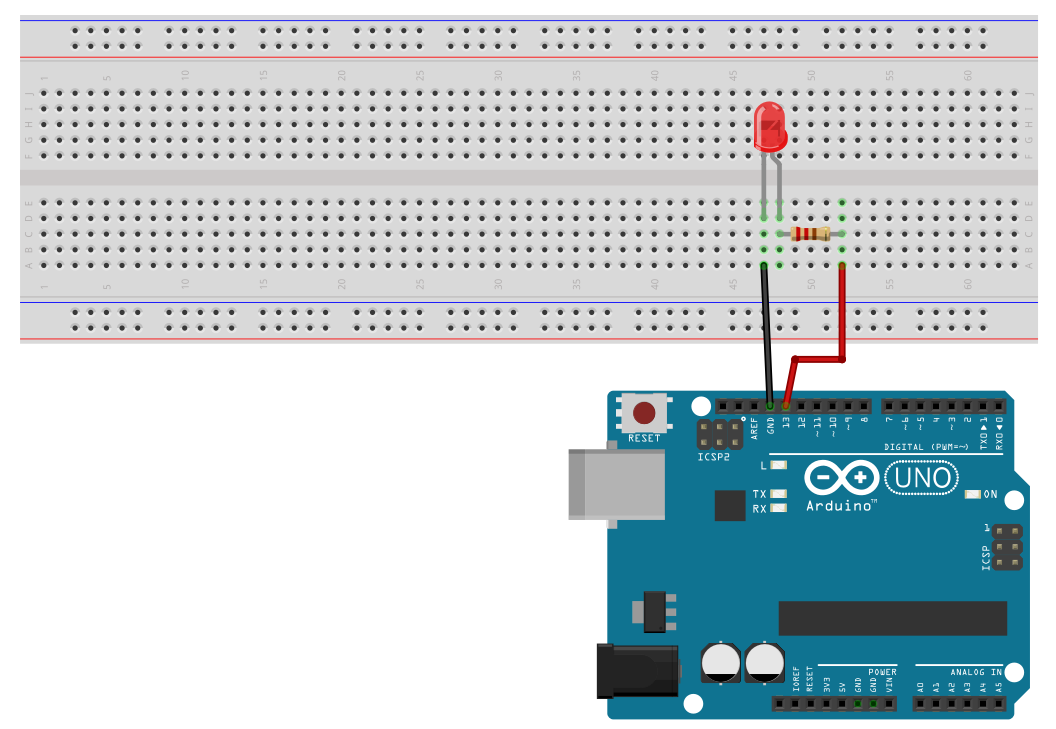
\includegraphics[height=3.5in]{lab_img/001_SimpleBlink.png}}
\label{ris:image}
\end{figure}

\begin{lstlisting}[label=lab01ex01,caption=Програмний код]
int LED = 13;

void setup() {
	pinMode(LED, OUTPUT);
}

void loop() {
	digitalWrite(LED, HIGH);
	delay(1000);
	digitalWrite(LED, LOW);
	delay(1000);	
}
\end{lstlisting}

\begin{figure}[h!]
\caption{Схема підключення}
\center{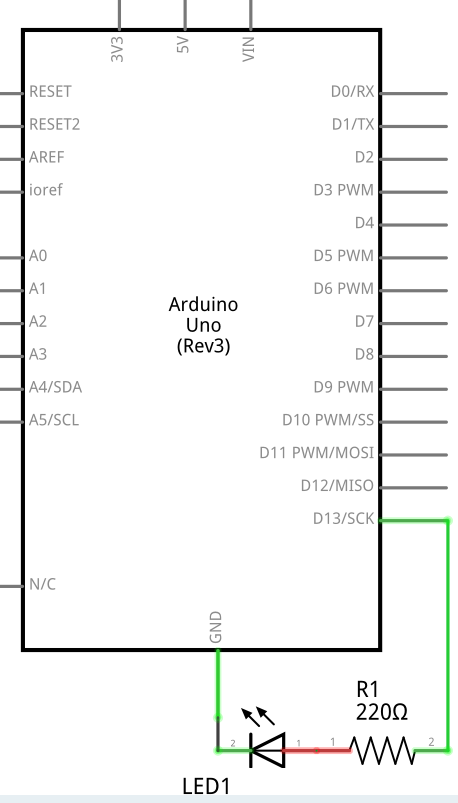
\includegraphics[height=4in]{lab_img/001_SimpleBlink_s.png}}
\label{ris:image}
\end{figure}

\section{ЛПР№2 [~Сигналізація~]}

\end{document}


